% Options for packages loaded elsewhere
\PassOptionsToPackage{unicode}{hyperref}
\PassOptionsToPackage{hyphens}{url}
\PassOptionsToPackage{dvipsnames,svgnames,x11names}{xcolor}
%
\documentclass[
  letterpaper,
  DIV=11,
  numbers=noendperiod]{scrartcl}
\usepackage{xcolor}
\usepackage{amsmath,amssymb}
\setcounter{secnumdepth}{-\maxdimen} % remove section numbering
\usepackage{iftex}
\ifPDFTeX
  \usepackage[T1]{fontenc}
  \usepackage[utf8]{inputenc}
  \usepackage{textcomp} % provide euro and other symbols
\else % if luatex or xetex
  \usepackage{unicode-math} % this also loads fontspec
  \defaultfontfeatures{Scale=MatchLowercase}
  \defaultfontfeatures[\rmfamily]{Ligatures=TeX,Scale=1}
\fi
\usepackage{lmodern}
\ifPDFTeX\else
  % xetex/luatex font selection
\fi
% Use upquote if available, for straight quotes in verbatim environments
\IfFileExists{upquote.sty}{\usepackage{upquote}}{}
\IfFileExists{microtype.sty}{% use microtype if available
  \usepackage[]{microtype}
  \UseMicrotypeSet[protrusion]{basicmath} % disable protrusion for tt fonts
}{}
\makeatletter
\@ifundefined{KOMAClassName}{% if non-KOMA class
  \IfFileExists{parskip.sty}{%
    \usepackage{parskip}
  }{% else
    \setlength{\parindent}{0pt}
    \setlength{\parskip}{6pt plus 2pt minus 1pt}}
}{% if KOMA class
  \KOMAoptions{parskip=half}}
\makeatother
% Make \paragraph and \subparagraph free-standing
\makeatletter
\ifx\paragraph\undefined\else
  \let\oldparagraph\paragraph
  \renewcommand{\paragraph}{
    \@ifstar
      \xxxParagraphStar
      \xxxParagraphNoStar
  }
  \newcommand{\xxxParagraphStar}[1]{\oldparagraph*{#1}\mbox{}}
  \newcommand{\xxxParagraphNoStar}[1]{\oldparagraph{#1}\mbox{}}
\fi
\ifx\subparagraph\undefined\else
  \let\oldsubparagraph\subparagraph
  \renewcommand{\subparagraph}{
    \@ifstar
      \xxxSubParagraphStar
      \xxxSubParagraphNoStar
  }
  \newcommand{\xxxSubParagraphStar}[1]{\oldsubparagraph*{#1}\mbox{}}
  \newcommand{\xxxSubParagraphNoStar}[1]{\oldsubparagraph{#1}\mbox{}}
\fi
\makeatother

\usepackage{color}
\usepackage{fancyvrb}
\newcommand{\VerbBar}{|}
\newcommand{\VERB}{\Verb[commandchars=\\\{\}]}
\DefineVerbatimEnvironment{Highlighting}{Verbatim}{commandchars=\\\{\}}
% Add ',fontsize=\small' for more characters per line
\usepackage{framed}
\definecolor{shadecolor}{RGB}{241,243,245}
\newenvironment{Shaded}{\begin{snugshade}}{\end{snugshade}}
\newcommand{\AlertTok}[1]{\textcolor[rgb]{0.68,0.00,0.00}{#1}}
\newcommand{\AnnotationTok}[1]{\textcolor[rgb]{0.37,0.37,0.37}{#1}}
\newcommand{\AttributeTok}[1]{\textcolor[rgb]{0.40,0.45,0.13}{#1}}
\newcommand{\BaseNTok}[1]{\textcolor[rgb]{0.68,0.00,0.00}{#1}}
\newcommand{\BuiltInTok}[1]{\textcolor[rgb]{0.00,0.23,0.31}{#1}}
\newcommand{\CharTok}[1]{\textcolor[rgb]{0.13,0.47,0.30}{#1}}
\newcommand{\CommentTok}[1]{\textcolor[rgb]{0.37,0.37,0.37}{#1}}
\newcommand{\CommentVarTok}[1]{\textcolor[rgb]{0.37,0.37,0.37}{\textit{#1}}}
\newcommand{\ConstantTok}[1]{\textcolor[rgb]{0.56,0.35,0.01}{#1}}
\newcommand{\ControlFlowTok}[1]{\textcolor[rgb]{0.00,0.23,0.31}{\textbf{#1}}}
\newcommand{\DataTypeTok}[1]{\textcolor[rgb]{0.68,0.00,0.00}{#1}}
\newcommand{\DecValTok}[1]{\textcolor[rgb]{0.68,0.00,0.00}{#1}}
\newcommand{\DocumentationTok}[1]{\textcolor[rgb]{0.37,0.37,0.37}{\textit{#1}}}
\newcommand{\ErrorTok}[1]{\textcolor[rgb]{0.68,0.00,0.00}{#1}}
\newcommand{\ExtensionTok}[1]{\textcolor[rgb]{0.00,0.23,0.31}{#1}}
\newcommand{\FloatTok}[1]{\textcolor[rgb]{0.68,0.00,0.00}{#1}}
\newcommand{\FunctionTok}[1]{\textcolor[rgb]{0.28,0.35,0.67}{#1}}
\newcommand{\ImportTok}[1]{\textcolor[rgb]{0.00,0.46,0.62}{#1}}
\newcommand{\InformationTok}[1]{\textcolor[rgb]{0.37,0.37,0.37}{#1}}
\newcommand{\KeywordTok}[1]{\textcolor[rgb]{0.00,0.23,0.31}{\textbf{#1}}}
\newcommand{\NormalTok}[1]{\textcolor[rgb]{0.00,0.23,0.31}{#1}}
\newcommand{\OperatorTok}[1]{\textcolor[rgb]{0.37,0.37,0.37}{#1}}
\newcommand{\OtherTok}[1]{\textcolor[rgb]{0.00,0.23,0.31}{#1}}
\newcommand{\PreprocessorTok}[1]{\textcolor[rgb]{0.68,0.00,0.00}{#1}}
\newcommand{\RegionMarkerTok}[1]{\textcolor[rgb]{0.00,0.23,0.31}{#1}}
\newcommand{\SpecialCharTok}[1]{\textcolor[rgb]{0.37,0.37,0.37}{#1}}
\newcommand{\SpecialStringTok}[1]{\textcolor[rgb]{0.13,0.47,0.30}{#1}}
\newcommand{\StringTok}[1]{\textcolor[rgb]{0.13,0.47,0.30}{#1}}
\newcommand{\VariableTok}[1]{\textcolor[rgb]{0.07,0.07,0.07}{#1}}
\newcommand{\VerbatimStringTok}[1]{\textcolor[rgb]{0.13,0.47,0.30}{#1}}
\newcommand{\WarningTok}[1]{\textcolor[rgb]{0.37,0.37,0.37}{\textit{#1}}}

\usepackage{longtable,booktabs,array}
\newcounter{none} % for unnumbered tables
\usepackage{calc} % for calculating minipage widths
% Correct order of tables after \paragraph or \subparagraph
\usepackage{etoolbox}
\makeatletter
\patchcmd\longtable{\par}{\if@noskipsec\mbox{}\fi\par}{}{}
\makeatother
% Allow footnotes in longtable head/foot
\IfFileExists{footnotehyper.sty}{\usepackage{footnotehyper}}{\usepackage{footnote}}
\makesavenoteenv{longtable}
\usepackage{graphicx}
\makeatletter
\newsavebox\pandoc@box
\newcommand*\pandocbounded[1]{% scales image to fit in text height/width
  \sbox\pandoc@box{#1}%
  \Gscale@div\@tempa{\textheight}{\dimexpr\ht\pandoc@box+\dp\pandoc@box\relax}%
  \Gscale@div\@tempb{\linewidth}{\wd\pandoc@box}%
  \ifdim\@tempb\p@<\@tempa\p@\let\@tempa\@tempb\fi% select the smaller of both
  \ifdim\@tempa\p@<\p@\scalebox{\@tempa}{\usebox\pandoc@box}%
  \else\usebox{\pandoc@box}%
  \fi%
}
% Set default figure placement to htbp
\def\fps@figure{htbp}
\makeatother

\setlength{\emergencystretch}{3em} % prevent overfull lines

\providecommand{\tightlist}{%
  \setlength{\itemsep}{0pt}\setlength{\parskip}{0pt}}

\usepackage{tikz}
\usetikzlibrary{positioning,arrows.meta,calc,shapes.geometric}
\KOMAoption{captions}{tableheading}
\makeatletter
\@ifpackageloaded{caption}{}{\usepackage{caption}}
\AtBeginDocument{%
\ifdefined\contentsname
  \renewcommand*\contentsname{Table des mati\`eres}
\else
  \newcommand\contentsname{Table des mati\`eres}
\fi
\ifdefined\listfigurename
  \renewcommand*\listfigurename{Liste des figures}
\else
  \newcommand\listfigurename{Liste des figures}
\fi
\ifdefined\listtablename
  \renewcommand*\listtablename{Liste des tableaux}
\else
  \newcommand\listtablename{Liste des tableaux}
\fi
\ifdefined\figurename
  \renewcommand*\figurename{Figure}
\else
  \newcommand\figurename{Figure}
\fi
\ifdefined\tablename
  \renewcommand*\tablename{Tableau}
\else
  \newcommand\tablename{Tableau}
\fi
}
\@ifpackageloaded{float}{}{\usepackage{float}}
\floatstyle{ruled}
\@ifundefined{c@chapter}{\newfloat{codelisting}{h}{lop}}{\newfloat{codelisting}{h}{lop}[chapter]}
\floatname{codelisting}{Listing}
\newcommand*\listoflistings{\listof{codelisting}{Liste des listings}}
\makeatother
\makeatletter
\makeatother
\makeatletter
\@ifpackageloaded{caption}{}{\usepackage{caption}}
\@ifpackageloaded{subcaption}{}{\usepackage{subcaption}}
\makeatother
\usepackage{bookmark}
\IfFileExists{xurl.sty}{\usepackage{xurl}}{} % add URL line breaks if available
\urlstyle{same}
\hypersetup{
  pdftitle={Reseau de Neurones en C sans bibliotheque -- TEI Sujet n.7},
  pdfauthor={IDIRENE Daris, MIZERKIN Nikita},
  colorlinks=true,
  linkcolor={blue},
  filecolor={Maroon},
  citecolor={Blue},
  urlcolor={Blue},
  pdfcreator={LaTeX via pandoc}}


\title{Reseau de Neurones en C sans bibliotheque \\ TEI Sujet n\textsuperscript{o}7}
\author{IDIRENE Daris, MIZERKIN Nikita}
\date{}
\begin{document}
\maketitle

\tableofcontents
\newpage

%% ============================================================
%% SECTION 1 : INTRODUCTION ET CONTEXTE
%% ============================================================
\subsection{1. Introduction et contexte du projet}\label{introduction-du-projet}

\subsubsection{1.1 Objectif}\label{objectif}

Ce projet consiste a implementer en C une bibliotheque \textbf{complete et auto-contenue} de reseaux de neurones denses (\emph{fully connected networks}), sans framework de machine learning externe. Le cas d'usage principal est la \textbf{classification des chiffres manuscrits MNIST}, ou chaque image de taille \(28\times 28\) pixels est vectorisee dans \(\mathbb{R}^{784}\) et classee parmi 10 categories (chiffres 0--9).

Le projet inclut egalement une \textbf{interface web} permettant de dessiner des chiffres et d'obtenir une prediction en temps reel, ainsi qu'un \textbf{pipeline CI/CD} pour l'integration continue sur GitLab.

\subsubsection{1.2 Architecture generale du projet}\label{architecture-generale-du-projet}

Le depot est organise autour du dossier \texttt{nn/} suivant une \textbf{separation modulaire stricte} :

\begin{verbatim}
nn/
+-- include/
|   +-- neuralnet.h        # Facade API publique
|   +-- nn/
|       +-- matrix.h       # Primitives d'algebre lineaire (vecteurs, matrices)
|       +-- nn_functions.h # Fonctions d'activation, pertes, optimiseurs
|       +-- network.h      # Architecture reseau et orchestration (forward/backprop)
|       +-- mnist.h        # Chargement PNG, cache binaire MNIST
+-- src/                   # Implementations C
|   +-- matrix.c
|   +-- nn_functions.c
|   +-- network.c
|   +-- mnist.c
+-- examples/              # Executables d'entrainement
+-- tests/                 # Tests unitaires (CTest)
+-- web/                   # Interface web de demonstration (Go + JavaScript)
\end{verbatim}

\subsubsection{1.3 Philosophie de conception}\label{philosophie-de-conception}

\begin{enumerate}
\def\labelenumi{\arabic{enumi}.}
\item
  \textbf{Zero malloc dans la boucle d'entrainement} : Les buffers de travail (deltas, activations, gradients) sont pre-alloues une seule fois lors de la creation du reseau, puis reutilises. Cela elimine la fragmentation memoire et garantit des performances previsibles.
\item
  \textbf{Separation couches vs primitives} :
  \begin{itemize}
  \tightlist
  \item
    \texttt{matrix.c} : produits matrice-vecteur efficaces
  \item
    \texttt{nn\_functions.c} : operations elementaires (activation, perte, gradient)
  \item
    \texttt{network.c} : orchestration forward/backward
  \end{itemize}
\item
  \textbf{Single-thread SGD} : Chaque epoque traite les 60\,000 images MNIST une par une avec mise a jour immediate des poids, sans batching ni parallelisation (pour simplicite).
\item
  \textbf{Configurabilite} : Le reseau supporte plusieurs fonctions d'activation (Sigmoid, ReLU, Tanh, Softmax, Leaky ReLU, Linear), fonctions de perte (MSE, MAE, BCE, CCE) et optimiseurs (SGD, Adam), configurables a l'execution via \texttt{nn\_network\_set\_training\_config()}.
\end{enumerate}

\subsubsection{1.4 Structure d'une couche reseau}\label{structure-dune-couche-reseau}

Chaque couche encapsule ses poids et ses caches locaux :

\begin{Shaded}
\begin{Highlighting}[]
\KeywordTok{typedef} \KeywordTok{struct} \OperatorTok{\{}
\NormalTok{    Matrix }\OperatorTok{*}\NormalTok{weights}\OperatorTok{;}        \CommentTok{// Poids W (biais integre via [W|b])}
\NormalTok{    Vector }\OperatorTok{*}\NormalTok{input\_cache}\OperatorTok{;}    \CommentTok{// Entree x mise en cache pour retroprop}
\NormalTok{    Vector }\OperatorTok{*}\NormalTok{output\_cache}\OperatorTok{;}   \CommentTok{// Sortie a = sigma(z) mise en cache}
\NormalTok{    Vector }\OperatorTok{*}\NormalTok{bias\_input}\OperatorTok{;}     \CommentTok{// Entree completee [x|1] pour mat-vec}
\OperatorTok{\}}\NormalTok{ Layer}\OperatorTok{;}
\end{Highlighting}
\end{Shaded}

\subsubsection{1.5 Representation des biais dans le code}\label{representation-des-biais}

\textbf{Convention : integration du biais en colonne augmentee}. Au lieu de stocker \(W\) et \(b\) separement, on cree :
\[\tilde{W} = \begin{bmatrix} W & b \end{bmatrix}, \quad \tilde{x} = \begin{bmatrix} x \\ 1 \end{bmatrix}\]
Alors \(z = \tilde{W} \tilde{x}\) en une seule operation mat-vec. Cela simplifie le code et ameliore la localite memoire.


%% ============================================================
%% SECTION 2 : ARCHITECTURE (DARIS -- NE PAS MODIFIER)
%% ============================================================
\subsection{2. Architecture d'un reseau de neurones : structure et visualisation}\label{architecture-dun-reseau-de-neurones}

\subsubsection{2.1 Diagramme d'un neurone unique}\label{diagramme-dun-neurone-unique}

Un neurone effectue une \textbf{combinaison lineaire} de ses entrees, puis applique une \textbf{fonction d'activation} :

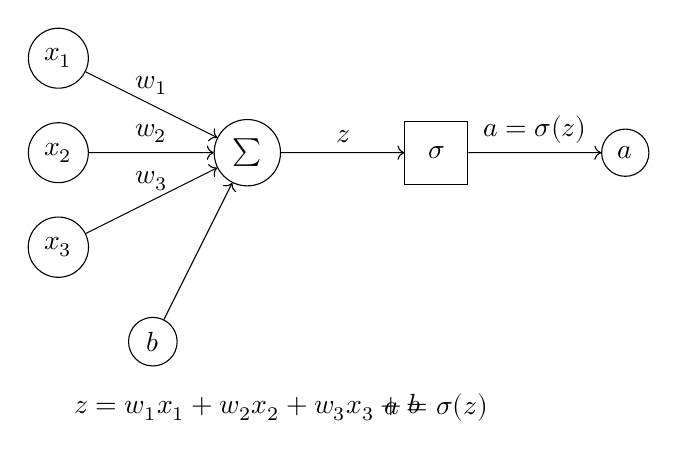
\begin{tikzpicture}[scale=1.2]
  % Entrees
  \node[circle, draw, minimum size=6mm] (x1) at (0, 1.5) {$x_1$};
  \node[circle, draw, minimum size=6mm] (x2) at (0, 0.5) {$x_2$};
  \node[circle, draw, minimum size=6mm] (x3) at (0, -0.5) {$x_3$};

  % Somme
  \node[circle, draw, minimum size=8mm] (sum) at (2, 0.5) {$\sum$};

  % Biais
  \node[circle, draw, minimum size=6mm] (b) at (1, -1.5) {$b$};

  % Activation
  \node[rectangle, draw, minimum size=8mm] (act) at (4, 0.5) {$\sigma$};

  % Sortie
  \node[circle, draw, minimum size=6mm] (out) at (6, 0.5) {$a$};

  % Connexions
  \draw[->] (x1) -- node[above] {$w_1$} (sum);
  \draw[->] (x2) -- node[above] {$w_2$} (sum);
  \draw[->] (x3) -- node[above] {$w_3$} (sum);
  \draw[->] (b) -- (sum);
  \draw[->] (sum) -- node[above] {$z$} (act);
  \draw[->] (act) -- node[above] {$a=\sigma(z)$} (out);

  % Formules
  \node at (2, -2.2) {$z = w_1 x_1 + w_2 x_2 + w_3 x_3 + b$};
  \node at (4, -2.2) {$a = \sigma(z)$};
\end{tikzpicture}

\subsubsection{2.2 Architecture d'un reseau complet}\label{architecture-dun-reseau-complet}

Pour MNIST, la structure typique est : \[784 \to 128 \to 64 \to 10\]

Soit : \textbf{entree 784D} (pixels) \(\to\) \textbf{couche cachee 128} (ReLU) \(\to\) \textbf{couche cachee 64} (ReLU) \(\to\) \textbf{sortie 10} (Softmax pour probabilites de classe).

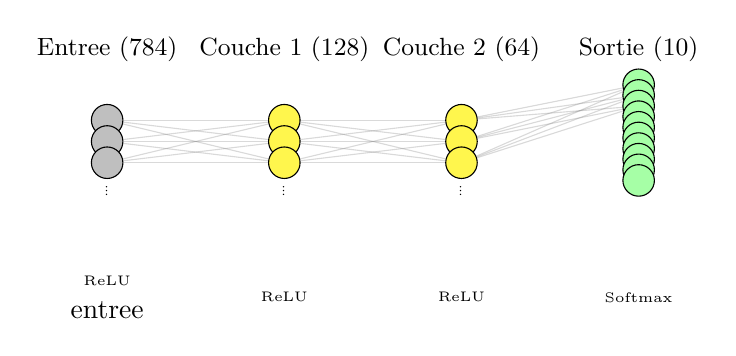
\begin{tikzpicture}[scale=0.9]
  % Couche d'entree (selection de quelques noeuds pour clarte)
  \node at (-2.5, 2.5) {\small Entree (784)};
  \foreach \i in {0, 1, 2} {
    \node[circle, draw, minimum size=4mm, fill=lightgray] (in\i) at (-2.5, 1.5 - 0.3*\i) {};
  }
  \node at (-2.5, 0.5) {\tiny $\vdots$};

  % Couche cachee 1 (128)
  \node at (0, 2.5) {\small Couche 1 (128)};
  \foreach \i in {0, 1, 2} {
    \node[circle, draw, minimum size=4mm, fill=yellow!70] (h1\i) at (0, 1.5 - 0.3*\i) {};
  }
  \node at (0, 0.5) {\tiny $\vdots$};

  % Couche cachee 2 (64)
  \node at (2.5, 2.5) {\small Couche 2 (64)};
  \foreach \i in {0, 1, 2} {
    \node[circle, draw, minimum size=4mm, fill=yellow!70] (h2\i) at (2.5, 1.5 - 0.3*\i) {};
  }
  \node at (2.5, 0.5) {\tiny $\vdots$};

  % Couche de sortie (10)
  \node at (5, 2.5) {\small Sortie (10)};
  \foreach \i in {0,...,9} {
    \node[circle, draw, minimum size=4mm, fill=green!35] (out\i) at (5, 2 - 0.15*\i) {};
  }

  % Connexions par couche
  \foreach \i in {0, 1, 2} {
    \foreach \j in {0, 1, 2} {
      \draw[gray, opacity=0.3] (in\i) -- (h1\j);
      \draw[gray, opacity=0.3] (h1\i) -- (h2\j);
      \draw[gray, opacity=0.3] (h2\i) -- (out\j);
    }
  }

  % Annotations
  \node[align=center] at (-2.5, -1) {\tiny ReLU \\ entree};
  \node[align=center] at (0, -1) {\tiny ReLU};
  \node[align=center] at (2.5, -1) {\tiny ReLU};
  \node[align=center] at (5, -1) {\tiny Softmax};
\end{tikzpicture}

\subsubsection{2.3 Representation mathematique}\label{representation-mathematique}

Pour un reseau a \(L\) couches parametrees (sans compter l'entree) :

\textbf{Notation des activations et pre-activations :}
\begin{itemize}
\tightlist
\item \(a^{(0)} = x \in \mathbb{R}^{n_0}\) : activation d'entree (image MNIST)
\item \(z^{(\ell)} \in \mathbb{R}^{n_\ell}\) : pre-activation couche \(\ell\)
\item \(a^{(\ell)} = \sigma_\ell(z^{(\ell)}) \in \mathbb{R}^{n_\ell}\) : activation couche \(\ell\)
\item \(W^{(\ell)} \in \mathbb{R}^{n_\ell \times n_{\ell-1}}\) : poids
\item \(b^{(\ell)} \in \mathbb{R}^{n_\ell}\) : biais
\end{itemize}

\textbf{Propagation avant (standard) :}
\[z^{(\ell)} = W^{(\ell)} a^{(\ell-1)} + b^{(\ell)}, \quad a^{(\ell)} = \sigma_\ell(z^{(\ell)})\]

\textbf{Avec representation augmentee (convention du code) :}
\[\tilde{a}^{(\ell-1)} = \begin{bmatrix} a^{(\ell-1)} \\ 1 \end{bmatrix}, \quad \tilde{W}^{(\ell)} = \begin{bmatrix} W^{(\ell)} & b^{(\ell)} \end{bmatrix}\]
\[z^{(\ell)} = \tilde{W}^{(\ell)} \tilde{a}^{(\ell-1)}\]

Cette astuce \textbf{elimine les boucles de biais} et ameliore la cache locality.

%% ============================================================
%% SECTION 3 : PROPAGATION AVANT (DARIS -- NE PAS MODIFIER)
%% ============================================================
\subsection{3. Propagation avant (\emph{Forward Pass}) : details et code}\label{propagation-avant}

\subsubsection{3.1 Pseudo-algorithme}\label{pseudo-algorithme}

\begin{verbatim}
function FORWARD(input):
    a[0] <- input
    for l from 1 to L:
        augment a[l-1] -> a~[l-1] (ajouter colonne de 1s)
        z[l] <- W[l] @ a~[l-1]          // mat-vec product
        if l < L:
            a[l] <- activation_hidden(z[l])
        else:
            a[l] <- activation_output(z[l])
    return a[L]   // prediction finale
\end{verbatim}

\subsubsection{3.2 Code C d'une propagation avant}\label{code-c-forward}

\begin{Shaded}
\begin{Highlighting}[]
\DataTypeTok{void}\NormalTok{ nn\_network\_forward}\OperatorTok{(}\DataTypeTok{const}\NormalTok{ Network }\OperatorTok{*}\NormalTok{network}\OperatorTok{,} \DataTypeTok{const}\NormalTok{ Vector }\OperatorTok{*}\NormalTok{input}\OperatorTok{)} \OperatorTok{\{}
    \CommentTok{// Placer l\textquotesingle{}entree dans le cache de la premiere couche}
\NormalTok{    copy\_vector}\OperatorTok{(}\NormalTok{input}\OperatorTok{,}\NormalTok{ network}\OperatorTok{{-}\textgreater{}}\NormalTok{layers}\OperatorTok{[}\DecValTok{0}\OperatorTok{]{-}\textgreater{}}\NormalTok{input\_cache}\OperatorTok{);}

    \ControlFlowTok{for} \OperatorTok{(}\DataTypeTok{size\_t}\NormalTok{ i }\OperatorTok{=} \DecValTok{0}\OperatorTok{;}\NormalTok{ i }\OperatorTok{\textless{}}\NormalTok{ network}\OperatorTok{{-}\textgreater{}}\NormalTok{num\_layers}\OperatorTok{;}\NormalTok{ i}\OperatorTok{++)} \OperatorTok{\{}
\NormalTok{        Layer }\OperatorTok{*}\NormalTok{layer }\OperatorTok{=}\NormalTok{ network}\OperatorTok{{-}\textgreater{}}\NormalTok{layers}\OperatorTok{[}\NormalTok{i}\OperatorTok{];}

        \CommentTok{// Augmenter l\textquotesingle{}entree avec une colonne de 1 (biais)}
\NormalTok{        memcpy}\OperatorTok{(}\NormalTok{layer}\OperatorTok{{-}\textgreater{}}\NormalTok{bias\_input}\OperatorTok{{-}\textgreater{}}\NormalTok{data}\OperatorTok{,}\NormalTok{ layer}\OperatorTok{{-}\textgreater{}}\NormalTok{input\_cache}\OperatorTok{{-}\textgreater{}}\NormalTok{data}\OperatorTok{,}
\NormalTok{               layer}\OperatorTok{{-}\textgreater{}}\NormalTok{input\_cache}\OperatorTok{{-}\textgreater{}}\NormalTok{size }\OperatorTok{*} \KeywordTok{sizeof}\OperatorTok{(}\DataTypeTok{float}\OperatorTok{));}
\NormalTok{        layer}\OperatorTok{{-}\textgreater{}}\NormalTok{bias\_input}\OperatorTok{{-}\textgreater{}}\NormalTok{data}\OperatorTok{[}\NormalTok{layer}\OperatorTok{{-}\textgreater{}}\NormalTok{input\_cache}\OperatorTok{{-}\textgreater{}}\NormalTok{size}\OperatorTok{]} \OperatorTok{=} \FloatTok{1.0}\BuiltInTok{f}\OperatorTok{;}

        \CommentTok{// Produit matrice-vecteur: z = W @ [x | 1]}
\NormalTok{        mat\_vec\_mul}\OperatorTok{(}\NormalTok{layer}\OperatorTok{{-}\textgreater{}}\NormalTok{weights}\OperatorTok{,}\NormalTok{ layer}\OperatorTok{{-}\textgreater{}}\NormalTok{bias\_input}\OperatorTok{,}\NormalTok{ layer}\OperatorTok{{-}\textgreater{}}\NormalTok{output\_cache}\OperatorTok{);}

        \CommentTok{// Appliquer l\textquotesingle{}activation appropriee}
        \ControlFlowTok{if} \OperatorTok{(}\NormalTok{i }\OperatorTok{+} \DecValTok{1} \OperatorTok{\textless{}}\NormalTok{ network}\OperatorTok{{-}\textgreater{}}\NormalTok{num\_layers}\OperatorTok{)} \OperatorTok{\{}
\NormalTok{            nn\_activation\_apply}\OperatorTok{(}\NormalTok{layer}\OperatorTok{{-}\textgreater{}}\NormalTok{output\_cache}\OperatorTok{,}\NormalTok{ network}\OperatorTok{{-}\textgreater{}}\NormalTok{hidden\_activation}\OperatorTok{);}
        \OperatorTok{\}} \ControlFlowTok{else} \OperatorTok{\{}
\NormalTok{            nn\_activation\_apply}\OperatorTok{(}\NormalTok{layer}\OperatorTok{{-}\textgreater{}}\NormalTok{output\_cache}\OperatorTok{,}\NormalTok{ network}\OperatorTok{{-}\textgreater{}}\NormalTok{output\_activation}\OperatorTok{);}
        \OperatorTok{\}}

        \CommentTok{// La sortie de cette couche devient l\textquotesingle{}entree de la suivante}
        \ControlFlowTok{if} \OperatorTok{(}\NormalTok{i }\OperatorTok{+} \DecValTok{1} \OperatorTok{\textless{}}\NormalTok{ network}\OperatorTok{{-}\textgreater{}}\NormalTok{num\_layers}\OperatorTok{)} \OperatorTok{\{}
\NormalTok{            copy\_vector}\OperatorTok{(}\NormalTok{layer}\OperatorTok{{-}\textgreater{}}\NormalTok{output\_cache}\OperatorTok{,}\NormalTok{ network}\OperatorTok{{-}\textgreater{}}\NormalTok{layers}\OperatorTok{[}\NormalTok{i }\OperatorTok{+} \DecValTok{1}\OperatorTok{]{-}\textgreater{}}\NormalTok{input\_cache}\OperatorTok{);}
        \OperatorTok{\}}
    \OperatorTok{\}}
\OperatorTok{\}}
\end{Highlighting}
\end{Shaded}

\textbf{Points cles :}
\begin{itemize}
\tightlist
\item \textbf{Zero malloc} : tous les vecteurs sont pre-alloues et reutilises
\item \textbf{Caches} : chaque couche conserve son entree et sa sortie pour la retroprop
\item \textbf{Localite memoire} : \texttt{memcpy} pour les entrees augmentees
\end{itemize}

\subsubsection{3.3 Complexite et performance}\label{complexite-et-performance}

Pour une image MNIST et architecture 784 $\to$ 128 $\to$ 64 $\to$ 10 :

\begin{itemize}
\tightlist
\item
  Multiplication 784-vers-128 : \(784 \times 128 = 100\,352\) FLOPs
\item
  Activation ReLU (128) : 128 comparaisons
\item
  Multiplication 128-vers-64 : \(128 \times 64 = 8\,192\) FLOPs
\item
  Activation ReLU (64) : 64 comparaisons
\item
  Multiplication 64-vers-10 : \(64 \times 10 = 640\) FLOPs
\item
  Activation Softmax (10) : 30 exponentielles + normalisations
\end{itemize}

\textbf{Total par sample par epoque :} \textasciitilde110k FLOPs (tres rapide sur processeur moderne)

%% ============================================================
%% SECTION 4 : RETROPROPAGATION (DARIS -- NE PAS MODIFIER)
%% ============================================================
\subsection{4. Retropropagation (\emph{Back Propagation}) : theorie et implementation}\label{retropropagation}

\subsubsection{4.1 Fondamentalement : la regle de chaine}\label{regle-de-chaine}

L'objectif est de calculer \(\frac{\partial \mathcal{L}}{\partial W^{(\ell)}}\) pour mettre a jour chaque couche.

On definit le \textbf{signal d'erreur} (\emph{delta}) de chaque couche :
\[\delta^{(\ell)} = \frac{\partial \mathcal{L}}{\partial z^{(\ell)}}\]

Ce signal propage l'erreur \textbf{de la sortie vers l'entree}.

\subsubsection{4.2 Derivation complete des deltas}\label{derivation-des-deltas}

\textbf{Couche de sortie ($\ell = L$) :}
\[\delta^{(L)} = \frac{\partial \mathcal{L}}{\partial a^{(L)}} \odot \sigma_L'(z^{(L)})\]

ou \(\odot\) est le produit element par element et \(\sigma_L'\) est la derivee.

\textbf{Simplification pour Softmax + Cross-Entropie (tres frequente) :}
\[\text{Si } a^{(L)} = \text{softmax}(z^{(L)}) \text{ et } \mathcal{L} = -\sum_i t_i \log a_i^{(L)}\]
\[\text{alors } \delta^{(L)} = a^{(L)} - t\]

Cette simplification est \textbf{implementee explicitement} dans le code :

\begin{Shaded}
\begin{Highlighting}[]
\ControlFlowTok{if} \OperatorTok{(}\NormalTok{network}\OperatorTok{{-}\textgreater{}}\NormalTok{output\_activation }\OperatorTok{==}\NormalTok{ ACTIVATION\_SOFTMAX }\OperatorTok{\&\&}
\NormalTok{    network}\OperatorTok{{-}\textgreater{}}\NormalTok{loss\_type }\OperatorTok{==}\NormalTok{ LOSS\_CATEGORICAL\_CROSS\_ENTROPY}\OperatorTok{)} \OperatorTok{\{}
    \CommentTok{// Forme directe sans appel a derivee d\textquotesingle{}activation}
    \ControlFlowTok{for} \OperatorTok{(}\DataTypeTok{size\_t}\NormalTok{ i }\OperatorTok{=} \DecValTok{0}\OperatorTok{;}\NormalTok{ i }\OperatorTok{\textless{}}\NormalTok{ output\_size}\OperatorTok{;}\NormalTok{ i}\OperatorTok{++)} \OperatorTok{\{}
\NormalTok{        network}\OperatorTok{{-}\textgreater{}}\NormalTok{work\_delta}\OperatorTok{{-}\textgreater{}}\NormalTok{data}\OperatorTok{[}\NormalTok{i}\OperatorTok{]} \OperatorTok{=}
\NormalTok{            network}\OperatorTok{{-}\textgreater{}}\NormalTok{layers}\OperatorTok{[}\NormalTok{network}\OperatorTok{{-}\textgreater{}}\NormalTok{num\_layers }\OperatorTok{{-}} \DecValTok{1}\OperatorTok{]{-}\textgreater{}}\NormalTok{output\_cache}\OperatorTok{{-}\textgreater{}}\NormalTok{data}\OperatorTok{[}\NormalTok{i}\OperatorTok{]}
            \OperatorTok{{-}}\NormalTok{ target\_vec}\OperatorTok{{-}\textgreater{}}\NormalTok{data}\OperatorTok{[}\NormalTok{i}\OperatorTok{];}
    \OperatorTok{\}}
\OperatorTok{\}} \ControlFlowTok{else} \OperatorTok{\{}
    \CommentTok{// Cas general : loss\textquotesingle{} * activation\textquotesingle{}}
\NormalTok{    nn\_loss\_gradient}\OperatorTok{(...);}
\NormalTok{    nn\_activation\_derivative}\OperatorTok{(...);}
    \ControlFlowTok{for} \OperatorTok{(}\DataTypeTok{size\_t}\NormalTok{ i }\OperatorTok{=} \DecValTok{0}\OperatorTok{;}\NormalTok{ i }\OperatorTok{\textless{}}\NormalTok{ output\_size}\OperatorTok{;}\NormalTok{ i}\OperatorTok{++)} \OperatorTok{\{}
\NormalTok{        network}\OperatorTok{{-}\textgreater{}}\NormalTok{work\_delta}\OperatorTok{{-}\textgreater{}}\NormalTok{data}\OperatorTok{[}\NormalTok{i}\OperatorTok{]} \OperatorTok{*=}\NormalTok{ network}\OperatorTok{{-}\textgreater{}}\NormalTok{work\_act\_deriv}\OperatorTok{{-}\textgreater{}}\NormalTok{data}\OperatorTok{[}\NormalTok{i}\OperatorTok{];}
    \OperatorTok{\}}
\OperatorTok{\}}
\end{Highlighting}
\end{Shaded}

\textbf{Couches cachees ($\ell < L$) :}
\[\delta^{(\ell)} = \left(W^{(\ell+1)\top} \delta^{(\ell+1)}\right) \odot \sigma_\ell'(z^{(\ell)})\]

\subsubsection{4.3 Gradients des parametres}\label{gradients-des-parametres}

Une fois \(\delta^{(\ell)}\) disponible :
\[\frac{\partial \mathcal{L}}{\partial W_{ij}^{(\ell)}} = \delta_i^{(\ell)} \cdot a_j^{(\ell-1)}\]

Sous forme matricielle :
\[\frac{\partial \mathcal{L}}{\partial W^{(\ell)}} = \delta^{(\ell)} (a^{(\ell-1)})^\top\]

ou avec representation augmentee :
\[\frac{\partial \mathcal{L}}{\partial \tilde{W}^{(\ell)}} = \delta^{(\ell)} (\tilde{a}^{(\ell-1)})^\top\]

\subsubsection{4.4 Pseudo-algorithme complet : retropropagation}\label{pseudo-algo-backprop}

\begin{verbatim}
function BACKWARD(input, target):
    FORWARD(input)  // calculer tous les z[l] et a[l]

    // Initialiser le delta de sortie
    d[L] <- loss_gradient(a[L], target) * act_deriv(z[L])

    // Propager l'erreur vers l'arriere
    for l from L-1 down to 1:
        d[l] <- (W[l+1]^T @ d[l+1]) * act_deriv(z[l])

    // Mettre a jour tous les poids
    for l from 1 to L:
        gradW[l] <- d[l] @ (a[l-1])^T     // gradient
        W[l] <- W[l] - learning_rate * gradW[l]
\end{verbatim}

\subsubsection{4.5 Code C : retropropagation complete}\label{code-c-backprop}

\begin{Shaded}
\begin{Highlighting}[]
\DataTypeTok{void}\NormalTok{ nn\_network\_backward}\OperatorTok{(}\NormalTok{Network }\OperatorTok{*}\NormalTok{network}\OperatorTok{,} \DataTypeTok{const}\NormalTok{ Vector }\OperatorTok{*}\NormalTok{input}\OperatorTok{,}
                         \DataTypeTok{const}\NormalTok{ Vector }\OperatorTok{*}\NormalTok{target}\OperatorTok{,} \DataTypeTok{float}\NormalTok{ learning\_rate}\OperatorTok{)} \OperatorTok{\{}
    \CommentTok{// Passe avant pour mettre en cache les activations}
\NormalTok{    nn\_network\_forward}\OperatorTok{(}\NormalTok{network}\OperatorTok{,}\NormalTok{ input}\OperatorTok{);}

    \CommentTok{// --- Etape 1: Delta de sortie ---}
    \DataTypeTok{size\_t}\NormalTok{ output\_size }\OperatorTok{=}\NormalTok{ network}\OperatorTok{{-}\textgreater{}}\NormalTok{layers}\OperatorTok{[}\NormalTok{network}\OperatorTok{{-}\textgreater{}}\NormalTok{num\_layers }\OperatorTok{{-}} \DecValTok{1}\OperatorTok{]{-}\textgreater{}}\NormalTok{output\_cache}\OperatorTok{{-}\textgreater{}}\NormalTok{size}\OperatorTok{;}
    \DataTypeTok{const}\NormalTok{ Vector }\OperatorTok{*}\NormalTok{target\_vec }\OperatorTok{=}\NormalTok{ target}\OperatorTok{;}
    \ControlFlowTok{if} \OperatorTok{(}\NormalTok{target}\OperatorTok{{-}\textgreater{}}\NormalTok{size }\OperatorTok{==} \DecValTok{1}\OperatorTok{)} \OperatorTok{\{}
\NormalTok{        nn\_one\_hot}\OperatorTok{((}\DataTypeTok{size\_t}\OperatorTok{)}\NormalTok{target}\OperatorTok{{-}\textgreater{}}\NormalTok{data}\OperatorTok{[}\DecValTok{0}\OperatorTok{],}\NormalTok{ output\_size}\OperatorTok{,}\NormalTok{ network}\OperatorTok{{-}\textgreater{}}\NormalTok{work\_one\_hot}\OperatorTok{);}
\NormalTok{        target\_vec }\OperatorTok{=}\NormalTok{ network}\OperatorTok{{-}\textgreater{}}\NormalTok{work\_one\_hot}\OperatorTok{;}
    \OperatorTok{\}}

    \CommentTok{// Cas simplifie: Softmax + CCE -> delta = predicted - target}
    \ControlFlowTok{if} \OperatorTok{(}\NormalTok{network}\OperatorTok{{-}\textgreater{}}\NormalTok{output\_activation }\OperatorTok{==}\NormalTok{ ACTIVATION\_SOFTMAX }\OperatorTok{\&\&}
\NormalTok{        network}\OperatorTok{{-}\textgreater{}}\NormalTok{loss\_type }\OperatorTok{==}\NormalTok{ LOSS\_CATEGORICAL\_CROSS\_ENTROPY}\OperatorTok{)} \OperatorTok{\{}
        \ControlFlowTok{for} \OperatorTok{(}\DataTypeTok{size\_t}\NormalTok{ i }\OperatorTok{=} \DecValTok{0}\OperatorTok{;}\NormalTok{ i }\OperatorTok{\textless{}}\NormalTok{ output\_size}\OperatorTok{;}\NormalTok{ i}\OperatorTok{++)} \OperatorTok{\{}
\NormalTok{            network}\OperatorTok{{-}\textgreater{}}\NormalTok{work\_delta}\OperatorTok{{-}\textgreater{}}\NormalTok{data}\OperatorTok{[}\NormalTok{i}\OperatorTok{]} \OperatorTok{=}
\NormalTok{                network}\OperatorTok{{-}\textgreater{}}\NormalTok{layers}\OperatorTok{[}\NormalTok{network}\OperatorTok{{-}\textgreater{}}\NormalTok{num\_layers }\OperatorTok{{-}} \DecValTok{1}\OperatorTok{]{-}\textgreater{}}\NormalTok{output\_cache}\OperatorTok{{-}\textgreater{}}\NormalTok{data}\OperatorTok{[}\NormalTok{i}\OperatorTok{]}
                \OperatorTok{{-}}\NormalTok{ target\_vec}\OperatorTok{{-}\textgreater{}}\NormalTok{data}\OperatorTok{[}\NormalTok{i}\OperatorTok{];}
        \OperatorTok{\}}
    \OperatorTok{\}} \ControlFlowTok{else} \OperatorTok{\{}
        \CommentTok{// Cas general}
\NormalTok{        nn\_loss\_gradient}\OperatorTok{(}\NormalTok{network}\OperatorTok{{-}\textgreater{}}\NormalTok{layers}\OperatorTok{[}\NormalTok{network}\OperatorTok{{-}\textgreater{}}\NormalTok{num\_layers }\OperatorTok{{-}} \DecValTok{1}\OperatorTok{]{-}\textgreater{}}\NormalTok{output\_cache}\OperatorTok{,}
\NormalTok{                        target\_vec}\OperatorTok{,}\NormalTok{ network}\OperatorTok{{-}\textgreater{}}\NormalTok{work\_delta}\OperatorTok{,}\NormalTok{ network}\OperatorTok{{-}\textgreater{}}\NormalTok{loss\_type}\OperatorTok{);}
\NormalTok{        nn\_activation\_derivative}\OperatorTok{(}\NormalTok{network}\OperatorTok{{-}\textgreater{}}\NormalTok{layers}\OperatorTok{[}\NormalTok{network}\OperatorTok{{-}\textgreater{}}\NormalTok{num\_layers }\OperatorTok{{-}} \DecValTok{1}\OperatorTok{]{-}\textgreater{}}\NormalTok{output\_cache}\OperatorTok{,}
\NormalTok{                                network}\OperatorTok{{-}\textgreater{}}\NormalTok{work\_act\_deriv}\OperatorTok{,}\NormalTok{ network}\OperatorTok{{-}\textgreater{}}\NormalTok{output\_activation}\OperatorTok{);}
        \ControlFlowTok{for} \OperatorTok{(}\DataTypeTok{size\_t}\NormalTok{ i }\OperatorTok{=} \DecValTok{0}\OperatorTok{;}\NormalTok{ i }\OperatorTok{\textless{}}\NormalTok{ output\_size}\OperatorTok{;}\NormalTok{ i}\OperatorTok{++)} \OperatorTok{\{}
\NormalTok{            network}\OperatorTok{{-}\textgreater{}}\NormalTok{work\_delta}\OperatorTok{{-}\textgreater{}}\NormalTok{data}\OperatorTok{[}\NormalTok{i}\OperatorTok{]} \OperatorTok{*=}\NormalTok{ network}\OperatorTok{{-}\textgreater{}}\NormalTok{work\_act\_deriv}\OperatorTok{{-}\textgreater{}}\NormalTok{data}\OperatorTok{[}\NormalTok{i}\OperatorTok{];}
        \OperatorTok{\}}
    \OperatorTok{\}}

    \CommentTok{// --- Etape 2: Ping-pong buffers pour eviter les allocations ---}
\NormalTok{    Vector }\OperatorTok{*}\NormalTok{delta      }\OperatorTok{=}\NormalTok{ network}\OperatorTok{{-}\textgreater{}}\NormalTok{work\_delta}\OperatorTok{;}
\NormalTok{    Vector }\OperatorTok{*}\NormalTok{next\_delta }\OperatorTok{=}\NormalTok{ network}\OperatorTok{{-}\textgreater{}}\NormalTok{work\_prev\_delta}\OperatorTok{;}

    \CommentTok{// --- Etape 3: Retropropagation a travers les couches ---}
    \ControlFlowTok{for} \OperatorTok{(}\DataTypeTok{size\_t}\NormalTok{ l }\OperatorTok{=}\NormalTok{ network}\OperatorTok{{-}\textgreater{}}\NormalTok{num\_layers}\OperatorTok{;}\NormalTok{ l }\OperatorTok{\textgreater{}} \DecValTok{0}\OperatorTok{;}\NormalTok{ l}\OperatorTok{{-}{-})} \OperatorTok{\{}
\NormalTok{        Layer }\OperatorTok{*}\NormalTok{layer }\OperatorTok{=}\NormalTok{ network}\OperatorTok{{-}\textgreater{}}\NormalTok{layers}\OperatorTok{[}\NormalTok{l }\OperatorTok{{-}} \DecValTok{1}\OperatorTok{];}
\NormalTok{        Vector }\OperatorTok{*}\NormalTok{current\_delta }\OperatorTok{=}\NormalTok{ delta}\OperatorTok{;}

        \CommentTok{// Si ce n\textquotesingle{}est pas la premiere couche, propager a la couche precedente}
        \ControlFlowTok{if} \OperatorTok{(}\NormalTok{l }\OperatorTok{\textgreater{}} \DecValTok{1}\OperatorTok{)} \OperatorTok{\{}
            \DataTypeTok{size\_t}\NormalTok{ prev\_size }\OperatorTok{=}\NormalTok{ layer}\OperatorTok{{-}\textgreater{}}\NormalTok{input\_cache}\OperatorTok{{-}\textgreater{}}\NormalTok{size}\OperatorTok{;}

            \CommentTok{// delta\_prev = W\^{}T @ delta (retro-produit)}
            \ControlFlowTok{for} \OperatorTok{(}\DataTypeTok{size\_t}\NormalTok{ i }\OperatorTok{=} \DecValTok{0}\OperatorTok{;}\NormalTok{ i }\OperatorTok{\textless{}}\NormalTok{ prev\_size}\OperatorTok{;}\NormalTok{ i}\OperatorTok{++)} \OperatorTok{\{}
\NormalTok{                next\_delta}\OperatorTok{{-}\textgreater{}}\NormalTok{data}\OperatorTok{[}\NormalTok{i}\OperatorTok{]} \OperatorTok{=} \FloatTok{0.0}\BuiltInTok{f}\OperatorTok{;}
                \ControlFlowTok{for} \OperatorTok{(}\DataTypeTok{size\_t}\NormalTok{ j }\OperatorTok{=} \DecValTok{0}\OperatorTok{;}\NormalTok{ j }\OperatorTok{\textless{}}\NormalTok{ layer}\OperatorTok{{-}\textgreater{}}\NormalTok{weights}\OperatorTok{{-}\textgreater{}}\NormalTok{rows}\OperatorTok{;}\NormalTok{ j}\OperatorTok{++)} \OperatorTok{\{}
\NormalTok{                    next\_delta}\OperatorTok{{-}\textgreater{}}\NormalTok{data}\OperatorTok{[}\NormalTok{i}\OperatorTok{]} \OperatorTok{+=}
\NormalTok{                        layer}\OperatorTok{{-}\textgreater{}}\NormalTok{weights}\OperatorTok{{-}\textgreater{}}\NormalTok{data}\OperatorTok{[}\NormalTok{j }\OperatorTok{*}\NormalTok{ layer}\OperatorTok{{-}\textgreater{}}\NormalTok{weights}\OperatorTok{{-}\textgreater{}}\NormalTok{cols }\OperatorTok{+}\NormalTok{ i}\OperatorTok{]}
                        \OperatorTok{*}\NormalTok{ current\_delta}\OperatorTok{{-}\textgreater{}}\NormalTok{data}\OperatorTok{[}\NormalTok{j}\OperatorTok{];}
                \OperatorTok{\}}
            \OperatorTok{\}}

            \CommentTok{// Multiplier par derivee d\textquotesingle{}activation couche precedente}
\NormalTok{            nn\_activation\_derivative}\OperatorTok{(}\NormalTok{layer}\OperatorTok{{-}\textgreater{}}\NormalTok{input\_cache}\OperatorTok{,}
\NormalTok{                                    network}\OperatorTok{{-}\textgreater{}}\NormalTok{work\_act\_deriv}\OperatorTok{,}
\NormalTok{                                    network}\OperatorTok{{-}\textgreater{}}\NormalTok{hidden\_activation}\OperatorTok{);}
            \ControlFlowTok{for} \OperatorTok{(}\DataTypeTok{size\_t}\NormalTok{ i }\OperatorTok{=} \DecValTok{0}\OperatorTok{;}\NormalTok{ i }\OperatorTok{\textless{}}\NormalTok{ prev\_size}\OperatorTok{;}\NormalTok{ i}\OperatorTok{++)} \OperatorTok{\{}
\NormalTok{                next\_delta}\OperatorTok{{-}\textgreater{}}\NormalTok{data}\OperatorTok{[}\NormalTok{i}\OperatorTok{]} \OperatorTok{*=}\NormalTok{ network}\OperatorTok{{-}\textgreater{}}\NormalTok{work\_act\_deriv}\OperatorTok{{-}\textgreater{}}\NormalTok{data}\OperatorTok{[}\NormalTok{i}\OperatorTok{];}
            \OperatorTok{\}}

            \CommentTok{// Ping-pong: echanger les pointeurs, AUCUN malloc !}
\NormalTok{            Vector }\OperatorTok{*}\NormalTok{tmp }\OperatorTok{=}\NormalTok{ delta}\OperatorTok{;}
\NormalTok{            delta       }\OperatorTok{=}\NormalTok{ next\_delta}\OperatorTok{;}
\NormalTok{            next\_delta  }\OperatorTok{=}\NormalTok{ tmp}\OperatorTok{;}
        \OperatorTok{\}}

        \CommentTok{// --- Etape 4: Mise a jour des poids (SGD ou Adam) ---}
        \ControlFlowTok{if} \OperatorTok{(}\NormalTok{network}\OperatorTok{{-}\textgreater{}}\NormalTok{optimizer\_type }\OperatorTok{==}\NormalTok{ OPTIMIZER\_ADAM }\OperatorTok{\&\&}\NormalTok{ network}\OperatorTok{{-}\textgreater{}}\NormalTok{adam\_opts}\OperatorTok{)} \OperatorTok{\{}
\NormalTok{            nn\_adam\_update}\OperatorTok{(}\NormalTok{network}\OperatorTok{{-}\textgreater{}}\NormalTok{adam\_opts}\OperatorTok{[}\NormalTok{l }\OperatorTok{{-}} \DecValTok{1}\OperatorTok{],}\NormalTok{ layer}\OperatorTok{{-}\textgreater{}}\NormalTok{weights}\OperatorTok{,}\NormalTok{ grad}\OperatorTok{);}
        \OperatorTok{\}} \ControlFlowTok{else} \OperatorTok{\{}
            \CommentTok{// SGD basique: W = W - lr * (delta @ x\^{}T)}
            \ControlFlowTok{for} \OperatorTok{(}\DataTypeTok{size\_t}\NormalTok{ i }\OperatorTok{=} \DecValTok{0}\OperatorTok{;}\NormalTok{ i }\OperatorTok{\textless{}}\NormalTok{ layer}\OperatorTok{{-}\textgreater{}}\NormalTok{weights}\OperatorTok{{-}\textgreater{}}\NormalTok{rows}\OperatorTok{;}\NormalTok{ i}\OperatorTok{++)} \OperatorTok{\{}
                \ControlFlowTok{for} \OperatorTok{(}\DataTypeTok{size\_t}\NormalTok{ j }\OperatorTok{=} \DecValTok{0}\OperatorTok{;}\NormalTok{ j }\OperatorTok{\textless{}}\NormalTok{ layer}\OperatorTok{{-}\textgreater{}}\NormalTok{weights}\OperatorTok{{-}\textgreater{}}\NormalTok{cols}\OperatorTok{;}\NormalTok{ j}\OperatorTok{++)} \OperatorTok{\{}
\NormalTok{                    layer}\OperatorTok{{-}\textgreater{}}\NormalTok{weights}\OperatorTok{{-}\textgreater{}}\NormalTok{data}\OperatorTok{[}\NormalTok{i }\OperatorTok{*}\NormalTok{ cols }\OperatorTok{+}\NormalTok{ j}\OperatorTok{]} \OperatorTok{{-}=}
\NormalTok{                        learning\_rate }\OperatorTok{*}\NormalTok{ current\_delta}\OperatorTok{{-}\textgreater{}}\NormalTok{data}\OperatorTok{[}\NormalTok{i}\OperatorTok{]} \OperatorTok{*}\NormalTok{ layer}\OperatorTok{{-}\textgreater{}}\NormalTok{bias\_input}\OperatorTok{{-}\textgreater{}}\NormalTok{data}\OperatorTok{[}\NormalTok{j}\OperatorTok{];}
                \OperatorTok{\}}
            \OperatorTok{\}}
        \OperatorTok{\}}
    \OperatorTok{\}}
\OperatorTok{\}}
\end{Highlighting}
\end{Shaded}

\textbf{Optimisations cles :}
\begin{enumerate}
\def\labelenumi{\arabic{enumi}.}
\tightlist
\item \textbf{Ping-pong buffers} : alternance entre \texttt{work\_delta} et \texttt{work\_prev\_delta} sans malloc
\item \textbf{Deltas pre-calcules} : softmax+CCE optimise en une seule soustraction
\item \textbf{Produit matrice transposee} : boucles explicites pour utiliser la cache L1
\end{enumerate}

%% ============================================================
%% SECTION 5 : FONCTIONS D'ACTIVATION (DARIS -- NE PAS MODIFIER)
%% ============================================================
\subsection{5. Fonctions d'activation et leurs derivees}\label{fonctions-dactivation}

\subsubsection{5.1 Sigmoide}\label{sigmoide}

\textbf{Definition :} \[\sigma(x) = \frac{1}{1 + e^{-x}}\]

\textbf{Derivee :} \[\sigma'(x) = \sigma(x)(1 - \sigma(x))\]

\textbf{Proprietes :}
\begin{itemize}
\tightlist
\item Plage : \((0, 1)\)
\item Probleme : gradient vanishing pour \(|x| \gg 0\)
\item \textbf{Stabilite numerique} : Le code limite l'entree a \([-500, 500]\) pour eviter les underflow/overflow d'exponentielle
\end{itemize}

\begin{Shaded}
\begin{Highlighting}[]
\DataTypeTok{void}\NormalTok{ nn\_sigmoid}\OperatorTok{(}\DataTypeTok{const}\NormalTok{ Vector }\OperatorTok{*}\NormalTok{input}\OperatorTok{,}\NormalTok{ Vector }\OperatorTok{*}\NormalTok{output}\OperatorTok{)} \OperatorTok{\{}
    \ControlFlowTok{for} \OperatorTok{(}\DataTypeTok{size\_t}\NormalTok{ i }\OperatorTok{=} \DecValTok{0}\OperatorTok{;}\NormalTok{ i }\OperatorTok{\textless{}}\NormalTok{ input}\OperatorTok{{-}\textgreater{}}\NormalTok{size}\OperatorTok{;}\NormalTok{ i}\OperatorTok{++)} \OperatorTok{\{}
        \DataTypeTok{float}\NormalTok{ x }\OperatorTok{=}\NormalTok{ input}\OperatorTok{{-}\textgreater{}}\NormalTok{data}\OperatorTok{[}\NormalTok{i}\OperatorTok{];}
        \ControlFlowTok{if} \OperatorTok{(}\NormalTok{x }\OperatorTok{\textgreater{}} \FloatTok{500.0}\BuiltInTok{f}\OperatorTok{)}\NormalTok{ x }\OperatorTok{=} \FloatTok{500.0}\BuiltInTok{f}\OperatorTok{;}
        \ControlFlowTok{if} \OperatorTok{(}\NormalTok{x }\OperatorTok{\textless{}} \OperatorTok{{-}}\FloatTok{500.0}\BuiltInTok{f}\OperatorTok{)}\NormalTok{ x }\OperatorTok{=} \OperatorTok{{-}}\FloatTok{500.0}\BuiltInTok{f}\OperatorTok{;}
\NormalTok{        output}\OperatorTok{{-}\textgreater{}}\NormalTok{data}\OperatorTok{[}\NormalTok{i}\OperatorTok{]} \OperatorTok{=} \FloatTok{1.0}\BuiltInTok{f} \OperatorTok{/} \OperatorTok{(}\FloatTok{1.0}\BuiltInTok{f} \OperatorTok{+}\NormalTok{ expf}\OperatorTok{({-}}\NormalTok{x}\OperatorTok{));}
    \OperatorTok{\}}
\OperatorTok{\}}
\end{Highlighting}
\end{Shaded}

\subsubsection{5.2 ReLU}\label{relu}

\textbf{Definition :} \[\text{ReLU}(x) = \max(0, x)\]

\textbf{Derivee :} \[\text{ReLU}'(x) = \mathbb{1}_{x > 0}\]

\subsubsection{5.3 Tanh}\label{tanh}

\[\tanh(x) = \frac{e^x - e^{-x}}{e^x + e^{-x}}, \quad \tanh'(x) = 1 - \tanh^2(x)\]

\subsubsection{5.4 Softmax}\label{softmax}

\[\text{softmax}(z)_i = \frac{e^{z_i - m}}{\sum_j e^{z_j - m}}, \quad m = \max_j z_j\]

%% ============================================================
%% SECTION 6 : FONCTIONS DE PERTE (DARIS -- NE PAS MODIFIER)
%% ============================================================
\subsection{6. Fonctions de perte}\label{fonctions-de-perte}

\subsubsection{6.1 MSE (Mean Squared Error)}\label{mse}

\[\mathcal{L}_{\text{MSE}} = \frac{1}{n} \sum_i (y_i - \hat{y}_i)^2, \quad \nabla = \frac{2}{n}(y - \hat{y})\]

\subsubsection{6.2 CCE (Categorical Cross-Entropy)}\label{cce}

\[\mathcal{L}_{\text{CCE}} = -\sum_i t_i \log p_i, \quad \nabla = -\frac{t}{p}\]

\textbf{Simplification Softmax+CCE :} \[\delta^{(L)} = \hat{y} - t\]

%% ============================================================
%% SECTION 7 : OPTIMISATION (DARIS -- NE PAS MODIFIER)
%% ============================================================
\subsection{7. Optimisation : SGD et Adam}\label{optimisation-sgd-adam}

\subsubsection{7.1 SGD}\label{sgd}

\[W_{t+1} = W_t - \eta \nabla_W \mathcal{L}_t\]

\subsubsection{7.2 Adam}\label{adam}

\[m_t = \beta_1 m_{t-1} + (1-\beta_1) g_t, \quad v_t = \beta_2 v_{t-1} + (1-\beta_2) g_t^2\]
\[W_{t+1} = W_t - \alpha \frac{\hat{m}_t}{\sqrt{\hat{v}_t} + \varepsilon}\]

ou \(\hat{m}_t = \frac{m_t}{1-\beta_1^t}\), \(\hat{v}_t = \frac{v_t}{1-\beta_2^t}\)

%% ============================================================
%% SECTION 8 : OPTIMISATIONS DE PERFORMANCE
%% ============================================================
\subsection{8. Optimisations de performance et allocation memoire}\label{optimisations-performance}

L'un des objectifs principaux du projet etait d'obtenir des performances elevees en C pur, sans recourir a des bibliotheques d'algebre lineaire externes (BLAS, etc.). Cette section detaille les techniques d'optimisation mises en oeuvre a differents niveaux.

\subsubsection{8.1 Architecture sans malloc dans la boucle d'entrainement}\label{sans-malloc}

\textbf{Probleme initial :} Dans les premieres versions du code, chaque iteration de la boucle d'entrainement allouait et liberait dynamiquement les vecteurs de deltas et de gradients. Avec 60\,000 images et 5 epoques, cela representait des millions d'appels \texttt{malloc}/\texttt{free}, provoquant une fragmentation memoire et une latence imprevisible.

\textbf{Solution :} Tous les buffers de travail sont \textbf{pre-alloues une seule fois} lors de la creation du reseau dans \texttt{nn\_network\_create()}. La structure \texttt{Network} contient 5 buffers de travail permanents :

\begin{Shaded}
\begin{Highlighting}[]
\CommentTok{// Tampons pre-alloues dans la structure Network}
\NormalTok{Vector }\OperatorTok{*}\NormalTok{work\_predicted}\OperatorTok{;}   \CommentTok{// Vecteur de prediction}
\NormalTok{Vector }\OperatorTok{*}\NormalTok{work\_one\_hot}\OperatorTok{;}    \CommentTok{// Encodage one-hot de la cible}
\NormalTok{Vector }\OperatorTok{*}\NormalTok{work\_delta}\OperatorTok{;}      \CommentTok{// Signal d\textquotesingle{}erreur courant}
\NormalTok{Vector }\OperatorTok{*}\NormalTok{work\_prev\_delta}\OperatorTok{;} \CommentTok{// Signal d\textquotesingle{}erreur precedent (ping-pong)}
\NormalTok{Vector }\OperatorTok{*}\NormalTok{work\_act\_deriv}\OperatorTok{;}  \CommentTok{// Derivee d\textquotesingle{}activation}
\end{Highlighting}
\end{Shaded}

De plus, chaque \texttt{Layer} contient ses propres caches pre-alloues (\texttt{input\_cache}, \texttt{output\_cache}, \texttt{bias\_input}), dimensionnes selon les tailles des couches. Les buffers \texttt{work\_delta} et \texttt{work\_prev\_delta} sont alloues a la taille \texttt{max\_size}, c'est-a-dire la taille de la plus grande couche du reseau, pour pouvoir accueillir n'importe quel vecteur de delta sans reallocation.

\textbf{Resultat :} \textbf{zero appel malloc/free} pendant toute la boucle d'entrainement, quelle que soit le nombre d'epoques ou d'images.

\subsubsection{8.2 Ping-pong buffers pour retropropagation}\label{ping-pong}

Pendant la retropropagation, chaque couche produit un nouveau vecteur de delta a partir du delta de la couche suivante. Au lieu d'allouer un nouveau vecteur a chaque couche, on utilise deux buffers pre-alloues (\texttt{work\_delta} et \texttt{work\_prev\_delta}) en alternance :

\begin{Shaded}
\begin{Highlighting}[]
\NormalTok{Vector }\OperatorTok{*}\NormalTok{delta      }\OperatorTok{=}\NormalTok{ network}\OperatorTok{{-}\textgreater{}}\NormalTok{work\_delta}\OperatorTok{;}
\NormalTok{Vector }\OperatorTok{*}\NormalTok{next\_delta }\OperatorTok{=}\NormalTok{ network}\OperatorTok{{-}\textgreater{}}\NormalTok{work\_prev\_delta}\OperatorTok{;}

\ControlFlowTok{for} \OperatorTok{(}\NormalTok{...}\OperatorTok{)} \OperatorTok{\{}  \CommentTok{// Boucle sur les couches (de L vers 1)}
    \CommentTok{// Calcul de next\_delta a partir de delta}
    \CommentTok{// ...}

    \CommentTok{// Echange des pointeurs (aucune copie, aucun malloc)}
\NormalTok{    Vector }\OperatorTok{*}\NormalTok{tmp }\OperatorTok{=}\NormalTok{ delta}\OperatorTok{;}
\NormalTok{    delta       }\OperatorTok{=}\NormalTok{ next\_delta}\OperatorTok{;}
\NormalTok{    next\_delta  }\OperatorTok{=}\NormalTok{ tmp}\OperatorTok{;}
\OperatorTok{\}}
\end{Highlighting}
\end{Shaded}

Cette technique est analogue au \emph{double buffering} en graphisme : un buffer est lu pendant que l'autre est ecrit, puis on les echange. Cout de l'echange : \textbf{3 affectations de pointeurs} (au lieu d'un \texttt{malloc} + \texttt{memcpy} + \texttt{free}).

\subsubsection{8.3 Optimisation du shuffle MNIST}\label{optimisation-shuffle}

Le melange du dataset a chaque epoque (voir section 9.5) implique de permuter deux images de 784 floats (3\,136 octets) par echange. Deux approches ont ete comparees :

\textbf{Version initiale} (echange element par element) : \textasciitilde88ms par epoque

\begin{Shaded}
\begin{Highlighting}[]
\ControlFlowTok{for} \OperatorTok{(}\DataTypeTok{size\_t}\NormalTok{ i }\OperatorTok{=} \DecValTok{0}\OperatorTok{;}\NormalTok{ i }\OperatorTok{\textless{}}\NormalTok{ MNIST\_IMAGE\_SIZE}\OperatorTok{;}\NormalTok{ i}\OperatorTok{++)} \OperatorTok{\{}
    \DataTypeTok{float}\NormalTok{ tmp }\OperatorTok{=}\NormalTok{ img1}\OperatorTok{[}\NormalTok{i}\OperatorTok{];}
\NormalTok{    img1}\OperatorTok{[}\NormalTok{i}\OperatorTok{]} \OperatorTok{=}\NormalTok{ img2}\OperatorTok{[}\NormalTok{i}\OperatorTok{];}
\NormalTok{    img2}\OperatorTok{[}\NormalTok{i}\OperatorTok{]} \OperatorTok{=}\NormalTok{ tmp}\OperatorTok{;}
\OperatorTok{\}}
\end{Highlighting}
\end{Shaded}

Cette boucle effectue 784 iterations avec 3 acces memoire par iteration (2\,352 acces au total par echange). Pour 60\,000 images, cela represente des dizaines de millions d'acces memoire non contigus.

\textbf{Version optimisee} (echange par \texttt{memcpy}) : \textasciitilde84ms par epoque

\begin{Shaded}
\begin{Highlighting}[]
\NormalTok{memcpy}\OperatorTok{(}\NormalTok{temp}\OperatorTok{,}\NormalTok{ img1}\OperatorTok{,}\NormalTok{ MNIST\_IMAGE\_SIZE }\OperatorTok{*} \KeywordTok{sizeof}\OperatorTok{(}\DataTypeTok{float}\OperatorTok{));}
\NormalTok{memcpy}\OperatorTok{(}\NormalTok{img1}\OperatorTok{,}\NormalTok{ img2}\OperatorTok{,}\NormalTok{ MNIST\_IMAGE\_SIZE }\OperatorTok{*} \KeywordTok{sizeof}\OperatorTok{(}\DataTypeTok{float}\OperatorTok{));}
\NormalTok{memcpy}\OperatorTok{(}\NormalTok{img2}\OperatorTok{,}\NormalTok{ temp}\OperatorTok{,}\NormalTok{ MNIST\_IMAGE\_SIZE }\OperatorTok{*} \KeywordTok{sizeof}\OperatorTok{(}\DataTypeTok{float}\OperatorTok{));}
\end{Highlighting}
\end{Shaded}

La fonction \texttt{memcpy} de la libc est optimisee pour les copies en bloc (utilise les instructions SIMD du processeur, alignement memoire, prefetching). Gain mesure : \textbf{3--5\%} par epoque.

\subsubsection{8.4 Drapeaux de compilation}\label{drapeaux-compilation}

Le choix des drapeaux de compilation a un impact majeur sur les performances du code mathematique :

\begin{itemize}
\tightlist
\item \textbf{\texttt{-O3}} (GCC/Clang) ou \textbf{\texttt{/O2}} (MSVC) : active les optimisations agressives (inlining, deroulement de boucles, vectorisation automatique)
\item \textbf{\texttt{-ffast-math}} / \textbf{\texttt{/fp:fast}} : autorise les reordonnements d'operations flottantes, permettant au compilateur de vectoriser les boucles de produit scalaire
\item \textbf{\texttt{-march=native}} (GCC/Clang) : genere du code specifique au processeur hote (utilise SSE/AVX si disponible)
\end{itemize}

L'absence de ces drapeaux (compilation en \texttt{-O0} par defaut) entrainait un ralentissement de \textbf{24x} (voir section 15.2). Cet ecart s'explique par le fait que les boucles internes du produit matrice-vecteur representent plus de 90\% du temps de calcul, et beneficient fortement de la vectorisation et de l'inlining.

\subsubsection{8.5 Stockage contigu des donnees}\label{stockage-contigu}

Les matrices de poids sont stockees en \textbf{row-major} dans un tableau \texttt{float*} contigu (\texttt{data[rows * cols]}), et non comme un tableau de pointeurs de lignes. Cela garantit la localite spatiale lors du produit matrice-vecteur : les elements d'une meme ligne sont adjacents en memoire, ce qui maximise l'utilisation du cache L1/L2 du processeur.

Le meme principe est applique au stockage des images MNIST (voir section 9.2) : un seul bloc contigu pour les 60\,000 images, eliminant la fragmentation memoire.

\subsubsection{8.6 Sauvegarde et chargement binaire du modele}\label{sauvegarde-modele}

Le modele entraine est sauvegarde en format binaire brut via \texttt{nn\_network\_save()} :

\begin{center}
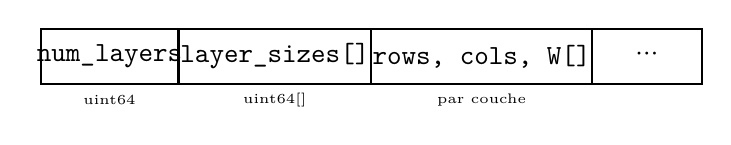
\begin{tikzpicture}[scale=0.7]
  \draw[thick] (0,0) rectangle (2.5,1);
  \node at (1.25, 0.5) {\texttt{num\_layers}};
  \node at (1.25, -0.3) {\tiny uint64};

  \draw[thick] (2.5,0) rectangle (6,1);
  \node at (4.25, 0.5) {\texttt{layer\_sizes[]}};
  \node at (4.25, -0.3) {\tiny uint64[]};

  \draw[thick] (6,0) rectangle (10,1);
  \node at (8, 0.5) {\texttt{rows, cols, W[]}};
  \node at (8, -0.3) {\tiny par couche};

  \draw[thick] (10,0) rectangle (12,1);
  \node at (11, 0.5) {$\cdots$};
\end{tikzpicture}
\end{center}

Ce format est directement lisible par le serveur Go (en little-endian), permettant le partage du modele entre le code d'entrainement C et le serveur d'inference Go sans conversion.

%% ============================================================
%% SECTION 9 : CHARGEMENT DES DONNEES MNIST
%% ============================================================
\subsection{9. Chargement des donnees MNIST}\label{chargement-mnist}

\subsubsection{9.1 Le dataset MNIST}\label{dataset-mnist}

Le dataset MNIST (\emph{Modified National Institute of Standards and Technology}) est un benchmark classique en apprentissage automatique. Il contient \textbf{70\,000 images de chiffres manuscrits} :
\begin{itemize}
\tightlist
\item \textbf{60\,000 images d'entrainement} (\emph{train set})
\item \textbf{10\,000 images de test} (\emph{test set})
\end{itemize}

Chaque image est en niveaux de gris, de taille \(28 \times 28\) pixels, soit \textbf{784 valeurs} par echantillon. Les chiffres sont centres et normalises dans l'image originale, ce qui constitue une convention importante a respecter lors de l'inference (voir section 10.2).

Nous utilisons la version decompressee en fichiers PNG individuels, organisee par repertoire selon l'etiquette :

\begin{verbatim}
mnist-pngs/
+-- train/
|   +-- 0/     # ~5923 images PNG du chiffre 0
|   +-- 1/     # ~6742 images PNG du chiffre 1
|   +-- ...
|   +-- 9/
+-- test/
    +-- 0/
    +-- ...
    +-- 9/
\end{verbatim}

Cette organisation par repertoire permet de deduire l'etiquette de chaque image directement a partir du nom de son repertoire parent, sans fichier d'index supplementaire.

\subsubsection{9.2 Structure de donnees}\label{structure-donnees-mnist}

\begin{Shaded}
\begin{Highlighting}[]
\KeywordTok{typedef} \KeywordTok{struct} \OperatorTok{\{}
\NormalTok{    }\DataTypeTok{float}\NormalTok{   }\OperatorTok{*}\NormalTok{images}\OperatorTok{;}      \CommentTok{// Donnees pixel normalisees (0.0-1.0)}
\NormalTok{    uint8\_t }\OperatorTok{*}\NormalTok{labels}\OperatorTok{;}      \CommentTok{// Etiquettes de classe (0-9)}
\NormalTok{    size\_t   count}\OperatorTok{;}       \CommentTok{// Nombre d\textquotesingle{}echantillons}
\OperatorTok{\}}\NormalTok{ mnist\_dataset\_t}\OperatorTok{;}
\end{Highlighting}
\end{Shaded}

Les images sont stockees dans un \textbf{tableau contigu unique} : l'image \(k\) commence a l'indice \texttt{k * 784}. Un seul \texttt{malloc} alloue l'ensemble du train set, conformement au principe de stockage contigu decrit en section 8.5.

Chaque pixel est normalise dans l'intervalle \([0, 1]\) par division par 255, transformant les valeurs entieres \texttt{uint8\_t} (0--255) en \texttt{float} (0.0--1.0). Cette normalisation est essentielle pour la convergence du reseau : des valeurs non normalisees provoqueraient des pre-activations \(z\) tres grandes, saturant les fonctions d'activation.

\subsubsection{9.3 Chargement depuis les PNG}\label{chargement-png}

Le chargement des PNG se fait en \textbf{deux passes} :

\textbf{Passe 1 -- Comptage :} La fonction \texttt{count\_files()} parcourt les 10 sous-repertoires (0 a 9) via l'API POSIX \texttt{opendir}/\texttt{readdir} pour determiner le nombre total d'images. Ce comptage prealable permet d'allouer exactement la memoire necessaire en un seul bloc.

\textbf{Passe 2 -- Chargement :} La fonction \texttt{mnist\_load\_dataset()} alloue la memoire (\texttt{count * 784} floats + \texttt{count} labels), puis parcourt a nouveau les repertoires pour charger chaque image.

Pour chaque fichier PNG, la fonction \texttt{mnist\_load\_png()} effectue le pipeline suivant :

\begin{enumerate}
\def\labelenumi{\arabic{enumi}.}
\tightlist
\item \textbf{Ouverture} du fichier en mode binaire (\texttt{fopen(..., "rb")})
\item \textbf{Initialisation libpng} : creation des structures \texttt{png\_structp} et \texttt{png\_infop}
\item \textbf{Gestion d'erreurs} : utilisation de \texttt{setjmp(png\_jmpbuf(png))} pour intercepter les erreurs de decodage PNG sans crash (libpng utilise des \emph{long jumps} pour sa gestion d'erreurs interne)
\item \textbf{Lecture des metadonnees} : dimensions de l'image via \texttt{png\_get\_image\_width/height()}
\item \textbf{Allocation et lecture} : allocation des pointeurs de lignes, puis \texttt{png\_read\_image()} pour decoder les pixels
\item \textbf{Normalisation} : conversion de chaque pixel \texttt{uint8} en \texttt{float} par division par 255.0
\item \textbf{Liberation} : desallocation des lignes, destruction des structures libpng, fermeture du fichier
\end{enumerate}

\begin{Shaded}
\begin{Highlighting}[]
\CommentTok{// Pipeline de decodage PNG simplifie}
\NormalTok{png\_structp png }\OperatorTok{=}\NormalTok{ png\_create\_read\_struct}\OperatorTok{(}\NormalTok{PNG\_LIBPNG\_VER\_STRING}\OperatorTok{,} \DataTypeTok{...}\OperatorTok{);}
\NormalTok{png\_infop info }\OperatorTok{=}\NormalTok{ png\_create\_info\_struct}\OperatorTok{(}\NormalTok{png}\OperatorTok{);}
\ControlFlowTok{if} \OperatorTok{(}\NormalTok{setjmp}\OperatorTok{(}\NormalTok{png\_jmpbuf}\OperatorTok{(}\NormalTok{png}\OperatorTok{)))}\NormalTok{  }\CommentTok{// Point de retour en cas d\textquotesingle{}erreur}
    \ControlFlowTok{return} \DecValTok{0}\OperatorTok{;}
\NormalTok{png\_read\_image}\OperatorTok{(}\NormalTok{png}\OperatorTok{,}\NormalTok{ row\_pointers}\OperatorTok{);}
\CommentTok{// Normalisation : uint8 -> float [0, 1]}
\ControlFlowTok{for} \OperatorTok{(}\DataTypeTok{int}\NormalTok{ y }\OperatorTok{=} \DecValTok{0}\OperatorTok{;}\NormalTok{ y }\OperatorTok{\textless{}}\NormalTok{ height}\OperatorTok{;}\NormalTok{ y}\OperatorTok{++)}
    \ControlFlowTok{for} \OperatorTok{(}\DataTypeTok{int}\NormalTok{ x }\OperatorTok{=} \DecValTok{0}\OperatorTok{;}\NormalTok{ x }\OperatorTok{\textless{}}\NormalTok{ width}\OperatorTok{;}\NormalTok{ x}\OperatorTok{++)}
\NormalTok{        out}\OperatorTok{[}\NormalTok{y }\OperatorTok{*}\NormalTok{ width }\OperatorTok{+}\NormalTok{ x}\OperatorTok{]} \OperatorTok{=}\NormalTok{ row\_pointers}\OperatorTok{[}\NormalTok{y}\OperatorTok{][}\NormalTok{x}\OperatorTok{]} \OperatorTok{/} \FloatTok{255.0}\BuiltInTok{f}\OperatorTok{;}
\end{Highlighting}
\end{Shaded}

\textbf{Probleme de performance :} Le chargement de 70\,000 fichiers PNG individuels prend \textbf{plus de 8 minutes}. Ce cout provient de trois facteurs cumules :
\begin{itemize}
\tightlist
\item \textbf{70\,000 appels systeme} \texttt{fopen}/\texttt{fclose} (creation de descripteurs de fichier)
\item \textbf{70\,000 decompressions DEFLATE} (le format PNG compresse les pixels via zlib)
\item \textbf{70\,000 allocations/liberations} des structures libpng et des buffers de lignes
\end{itemize}
Cette latence rendait le cycle de developpement extremement lent, chaque test necessitant plus de 8 minutes avant meme de commencer l'entrainement.

\subsubsection{9.4 Cache binaire}\label{cache-binaire}

Pour resoudre le probleme de temps de chargement, un systeme de \textbf{cache binaire} a ete implemente. L'idee est simple : apres le premier chargement depuis les PNG, les donnees normalisees sont sauvegardees dans un fichier binaire brut. Les lancements suivants chargent directement ce fichier en un seul appel \texttt{fread()}, sans decompression ni conversion.

Le format du cache est volontairement minimaliste et sequentiel :

\begin{center}
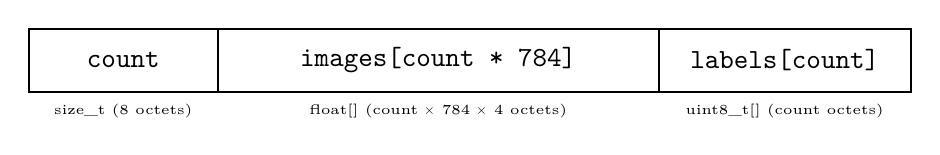
\begin{tikzpicture}[scale=0.8]
  \draw[thick] (0,0) rectangle (3,1);
  \node at (1.5, 0.5) {\texttt{count}};
  \node at (1.5, -0.3) {\tiny size\_t (8 octets)};

  \draw[thick] (3,0) rectangle (10,1);
  \node at (6.5, 0.5) {\texttt{images[count * 784]}};
  \node at (6.5, -0.3) {\tiny float[] (count $\times$ 784 $\times$ 4 octets)};

  \draw[thick] (10,0) rectangle (14,1);
  \node at (12, 0.5) {\texttt{labels[count]}};
  \node at (12, -0.3) {\tiny uint8\_t[] (count octets)};
\end{tikzpicture}
\end{center}

\textbf{Ecriture du cache} (\texttt{mnist\_save\_binary()}) :
\begin{Shaded}
\begin{Highlighting}[]
\NormalTok{fwrite}\OperatorTok{(\&}\NormalTok{dataset}\OperatorTok{{-}\textgreater{}}\NormalTok{count}\OperatorTok{,} \KeywordTok{sizeof}\OperatorTok{(}\NormalTok{size\_t}\OperatorTok{),} \DecValTok{1}\OperatorTok{,}\NormalTok{ f}\OperatorTok{);}
\NormalTok{fwrite}\OperatorTok{(}\NormalTok{dataset}\OperatorTok{{-}\textgreater{}}\NormalTok{images}\OperatorTok{,} \KeywordTok{sizeof}\OperatorTok{(}\DataTypeTok{float}\OperatorTok{),}\NormalTok{ count }\OperatorTok{*} \DecValTok{784}\OperatorTok{,}\NormalTok{ f}\OperatorTok{);}
\NormalTok{fwrite}\OperatorTok{(}\NormalTok{dataset}\OperatorTok{{-}\textgreater{}}\NormalTok{labels}\OperatorTok{,} \KeywordTok{sizeof}\OperatorTok{(}\NormalTok{uint8\_t}\OperatorTok{),}\NormalTok{ count}\OperatorTok{,}\NormalTok{ f}\OperatorTok{);}
\end{Highlighting}
\end{Shaded}

Le format n'utilise ni compression, ni en-tete de version, ni somme de controle. La structure en memoire est directement ecrite sur disque via \texttt{fwrite()}, ce qui signifie que le fichier cache est \textbf{specifique a la plateforme} (endianness, taille de \texttt{size\_t}). En pratique, cela ne pose pas de probleme car le cache est toujours genere et lu sur la meme machine.

\textbf{Tailles des fichiers cache :}
\begin{itemize}
\tightlist
\item \texttt{train.bin} : \(60\,000 \times 784 \times 4 + 60\,000 + 8 \approx \textbf{180 Mo}\)
\item \texttt{test.bin} : \(10\,000 \times 784 \times 4 + 10\,000 + 8 \approx \textbf{30 Mo}\)
\end{itemize}

\textbf{Lecture du cache} (\texttt{mnist\_load\_binary()}) : un seul \texttt{fread()} par champ, sans boucle ni conversion. Le systeme d'exploitation peut utiliser le \emph{readahead} pour prefetcher les donnees en lecture sequentielle.

\textbf{Impact sur les performances :} Le chargement binaire prend \textbf{quelques secondes} au lieu de plus de 8 minutes, soit un gain de l'ordre de \textbf{100x a 1000x} selon le disque. Ce gain provient de l'elimination complete de la decompression PNG, de la reduction du nombre d'appels systeme (3 au lieu de 70\,000), et de l'acces sequentiel optimise au fichier cache.

\textbf{Strategie d'utilisation dans les exemples :} Les programmes d'entrainement (\\texttt{examples/}) tentent d'abord de charger le cache binaire. Si celui-ci n'existe pas, ils chargent les PNG, puis sauvegardent le cache pour les lancements futurs.

\subsubsection{9.5 Melange du dataset}\label{melange-dataset}

Le melange (\emph{shuffle}) du dataset a chaque epoque est necessaire pour eviter que le reseau n'apprenne l'ordre des echantillons. Sans shuffle, les images etant groupees par etiquette (tous les 0, puis tous les 1, etc.), le reseau convergerait vers un biais en faveur de la derniere classe vue.

L'algorithme utilise est celui de \textbf{Fisher-Yates} (\emph{Knuth shuffle}), qui garantit un melange uniformement aleatoire en \(\mathcal{O}(n)\). L'optimisation des echanges d'images (784 floats par echange) est detaillee en section 8.3.

%% ============================================================
%% SECTION 10 : INTERFACE WEB
%% ============================================================
\subsection{10. Interface web de demonstration}\label{interface-web}

\subsubsection{10.1 Architecture generale}\label{archi-web}

L'interface web permet de dessiner un chiffre a la souris (ou au doigt sur mobile) et d'obtenir une prediction en temps reel. Elle est composee de deux parties distinctes :

\begin{itemize}
\tightlist
\item \textbf{Backend} : serveur Go utilisant le framework Gin, qui charge le modele pre-entraine au demarrage et effectue l'inference a chaque requete
\item \textbf{Frontend} : page HTML/CSS/JavaScript avec un canvas de dessin, un apercu de l'entree du modele, et des barres de confiance par classe
\end{itemize}

Le choix de Go pour le serveur (plutot qu'un binding C direct) permet un deploiement simple sans compilation croisee, tout en gardant une inference rapide grace a l'implementation en Go pur de la propagation avant.

\begin{center}
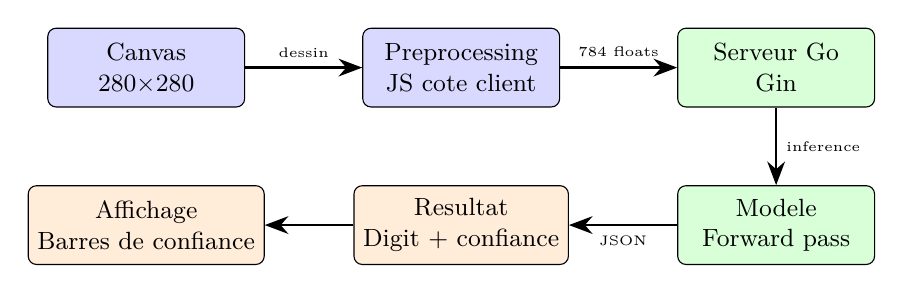
\begin{tikzpicture}[
  box/.style={rectangle, draw, rounded corners=3pt, minimum width=2.5cm, minimum height=1cm, align=center, font=\small},
  arrow/.style={-{Stealth[length=3mm]}, thick}
]
  \node[box, fill=blue!15] (canvas) at (0, 0) {Canvas\\280$\times$280};
  \node[box, fill=blue!15] (preprocess) at (4, 0) {Preprocessing\\JS cote client};
  \node[box, fill=green!15] (server) at (8, 0) {Serveur Go\\Gin};
  \node[box, fill=green!15] (model) at (8, -2) {Modele\\Forward pass};
  \node[box, fill=orange!15] (result) at (4, -2) {Resultat\\Digit + confiance};
  \node[box, fill=orange!15] (display) at (0, -2) {Affichage\\Barres de confiance};

  \draw[arrow] (canvas) -- node[above, font=\tiny] {dessin} (preprocess);
  \draw[arrow] (preprocess) -- node[above, font=\tiny] {784 floats} (server);
  \draw[arrow] (server) -- node[right, font=\tiny] {inference} (model);
  \draw[arrow] (model) -- node[below, font=\tiny] {JSON} (result);
  \draw[arrow] (result) -- (display);
\end{tikzpicture}
\end{center}

\subsubsection{10.2 Preprocessing cote client}\label{preprocessing-client}

Le preprocessing est l'etape la plus critique de l'interface web. Un chiffre dessine librement par l'utilisateur ne ressemble pas directement a une image MNIST : il peut etre trop grand, trop petit, decentre, ou positionne dans un coin du canvas. Le preprocessing doit \textbf{reproduire la normalisation appliquee aux images MNIST originales} pour que le modele recoive une entree coherente avec ses donnees d'entrainement.

Le pipeline de preprocessing en JavaScript suit 6 etapes :

\begin{enumerate}
\def\labelenumi{\arabic{enumi}.}
\item \textbf{Dessin} : l'utilisateur dessine sur un canvas de 280$\times$280 pixels (fond noir, trait blanc, epaisseur 22px). La taille 280$\times$280 correspond a un facteur 10$\times$ par rapport a 28$\times$28, offrant une resolution confortable pour le dessin.

\item \textbf{Boite englobante} (\emph{bounding box}) : parcours de tous les pixels du canvas pour trouver les coordonnees extremes du contenu dessine (\texttt{minX}, \texttt{minY}, \texttt{maxX}, \texttt{maxY}). Seuls les pixels dont l'intensite depasse un seuil de 10 (sur 255) sont consideres, filtrant ainsi le bruit de fond.

\item \textbf{Centre de masse} : calcul du barycentre pondere par l'intensite de chaque pixel :
\[x_{\text{cm}} = \frac{\sum_{(x,y)} x \cdot I(x,y)}{\sum_{(x,y)} I(x,y)}, \quad y_{\text{cm}} = \frac{\sum_{(x,y)} y \cdot I(x,y)}{\sum_{(x,y)} I(x,y)}\]
ou \(I(x,y)\) est l'intensite du pixel. Ce calcul est effectue simultanement avec la detection de la boite englobante, en une seule passe sur les pixels.

\item \textbf{Mise a l'echelle} : le contenu de la boite englobante est redimensionne pour tenir dans une zone de \textbf{20$\times$20 pixels}, en conservant le rapport d'aspect. Le facteur d'echelle est : \(\text{scale} = 20 / \max(\text{largeur}, \text{hauteur})\).

\item \textbf{Centrage par centre de masse} : le chiffre est positionne de sorte que son centre de masse se trouve au pixel \((14, 14)\) dans l'image 28$\times$28 finale. C'est cette etape qui reproduit la \textbf{convention MNIST originale} : les chiffres du dataset sont centres par leur centre de masse, pas par leur boite englobante.

\item \textbf{Normalisation} : extraction des pixels du canvas redimensionne et division par 255 pour obtenir des valeurs \texttt{float32} dans \([0, 1]\).
\end{enumerate}

Un canvas d'apercu (\texttt{28$\times$28} pixels, affiche en \texttt{56$\times$56}) permet a l'utilisateur de voir exactement l'image envoyee au modele, facilitant le diagnostic des erreurs de prediction.

\subsubsection{10.3 Compatibilite tactile}\label{compatibilite-tactile}

Le canvas gere les evenements tactiles (\texttt{touchstart}, \texttt{touchmove}, \texttt{touchend}) en plus des evenements souris, permettant l'utilisation sur tablettes et smartphones. Les coordonnees tactiles sont converties en coordonnees canvas via \texttt{getBoundingClientRect()}, et \texttt{preventDefault()} est appele pour empecher le defilement de la page pendant le dessin.

\subsubsection{10.4 Serveur Go et API}\label{serveur-go}

Le serveur Go utilise le framework \textbf{Gin} en mode Release (logs minimaux). Au demarrage, il charge le modele binaire en memoire, puis ecoute sur le port \textbf{4343} (configurable via \texttt{-{}-addr}). Le chemin du modele est configurable via \texttt{-{}-model}.

Le serveur expose deux endpoints :
\begin{itemize}
\tightlist
\item \texttt{GET /} : sert l'interface HTML depuis le repertoire \texttt{templates/}
\item \texttt{POST /api/predict} : recoit un tableau de 784 floats en JSON et retourne la prediction
\end{itemize}

L'endpoint de prediction effectue une \textbf{validation stricte} : le serveur rejette les requetes dont le tableau \texttt{pixels} ne contient pas exactement 784 elements, renvoyant une erreur HTTP 400 avec un message explicatif.

\begin{Shaded}
\begin{Highlighting}[]
\KeywordTok{type}\NormalTok{ PredictRequest }\KeywordTok{struct}\NormalTok{ \{}
\NormalTok{    Pixels []}\DataTypeTok{float32}\NormalTok{ }\StringTok{`json:"pixels" binding:"required"`}
\NormalTok{\}}

\KeywordTok{type}\NormalTok{ PredictResponse }\KeywordTok{struct}\NormalTok{ \{}
\NormalTok{    Digit      }\DataTypeTok{int}\NormalTok{       }\StringTok{`json:"digit"`}
\NormalTok{    Confidence []}\DataTypeTok{float32}\NormalTok{ }\StringTok{`json:"confidence"`}
\NormalTok{\}}
\end{Highlighting}
\end{Shaded}

La reponse contient le chiffre predit (\texttt{digit}) et le vecteur complet des 10 probabilites (\texttt{confidence}), permettant au frontend d'afficher les barres de confiance pour chaque classe.

\subsubsection{10.5 Inference en Go pur}\label{inference-go}

Le choix d'implementer l'inference \textbf{en Go pur} (sans \texttt{cgo}) est motive par la simplicite de deploiement : pas besoin de compiler la bibliotheque C sur la machine cible, pas de dependances dynamiques, un seul binaire Go suffit.

\textbf{Chargement du modele :} La fonction \texttt{LoadModel()} lit le fichier binaire produit par \texttt{nn\_network\_save()} en C. Toutes les valeurs sont lues en \textbf{little-endian} via le package \texttt{encoding/binary} de Go. La structure lue est identique a celle decrite en section 8.6 : nombre de couches, tailles, puis pour chaque couche les dimensions et les poids.

\textbf{Propagation avant :} Pour chaque couche, l'inference suit le meme algorithme que le code C :
\begin{enumerate}
\def\labelenumi{\arabic{enumi}.}
\tightlist
\item Construction de l'entree augmentee : \(\tilde{x} = [x \mid 1]\)
\item Produit matrice-vecteur : \(z = \tilde{W} \tilde{x}\)
\item Application de la sigmoide avec clampage dans \([-500, 500]\) (meme stabilite numerique que le code C)
\end{enumerate}

\begin{Shaded}
\begin{Highlighting}[]
\KeywordTok{func}\NormalTok{ (net *Network) }\FunctionTok{Predict}\NormalTok{(input []}\DataTypeTok{float32}\NormalTok{) (}\DataTypeTok{int}\NormalTok{, []}\DataTypeTok{float32}\NormalTok{) \{}
\NormalTok{    current := input}
    \ControlFlowTok{for}\NormalTok{ \_, layer := }\ControlFlowTok{range}\NormalTok{ net.Layers \{}
\NormalTok{        biasInput := }\BuiltInTok{make}\NormalTok{([]}\DataTypeTok{float32}\NormalTok{, }\BuiltInTok{len}\NormalTok{(current)+1)}
        \BuiltInTok{copy}\NormalTok{(biasInput, current)}
\NormalTok{        biasInput[}\BuiltInTok{len}\NormalTok{(current)] = }\FloatTok{1.0}
\NormalTok{        output := }\BuiltInTok{make}\NormalTok{([]}\DataTypeTok{float32}\NormalTok{, layer.Rows)}
        \ControlFlowTok{for}\NormalTok{ i := }\DecValTok{0}\NormalTok{; i < layer.Rows; i++ \{}
            \KeywordTok{var}\NormalTok{ sum }\DataTypeTok{float32}
            \ControlFlowTok{for}\NormalTok{ j := }\DecValTok{0}\NormalTok{; j < layer.Cols; j++ \{}
\NormalTok{                sum += layer.Weights[i*layer.Cols+j] * biasInput[j]}
\NormalTok{            \}}
\NormalTok{            output[i] = }\FunctionTok{sigmoid}\NormalTok{(sum)}
\NormalTok{        \}}
\NormalTok{        current = output}
\NormalTok{    \}}
    \ControlFlowTok{return} \FunctionTok{argmax}\NormalTok{(current), current}
\NormalTok{\}}
\end{Highlighting}
\end{Shaded}

L'interface web utilise le modele entraine avec \textbf{Sigmoid/MSE/SGD} (fichier \texttt{mnist\_model.bin}). Le choix de Sigmoid (plutot que Softmax) pour le serveur Go simplifie l'implementation : une seule fonction d'activation a implementer. Les sorties sigmoides ne sont pas de vraies probabilites (elles ne somment pas a 1), mais suffisent pour determiner le chiffre le plus probable via \texttt{argmax}.


%% ============================================================
%% SECTION 11 : TESTS
%% ============================================================
\subsection{11. Tests unitaires et validation}\label{tests}

Le projet utilise \textbf{CTest} (integre a CMake) pour l'execution automatisee des tests. Cinq suites couvrent les differentes couches du code :

\begin{itemize}
\tightlist
\item \textbf{test\_matrix} : primitives d'algebre lineaire (produit scalaire, mat-vec, transposition), tolerance \(\varepsilon = 10^{-6}\)
\item \textbf{test\_activation} : fonctions d'activation, de perte et leurs derivees, optimiseur Adam
\item \textbf{test\_network} : integration complete (creation, forward, entrainement sur le probleme OR)
\item \textbf{test\_mnist\_cnn\_system} : benchmark MNIST sur sous-ensemble reduit (2\,500 train / 800 test)
\item \textbf{test\_interactive} : test visuel exclu de CTest (affichage ASCII, prediction manuelle)
\end{itemize}

%% ============================================================
%% SECTION 12 : CI/CD
%% ============================================================
\subsection{12. Integration continue (CI/CD)}\label{cicd}

Le projet utilise \textbf{GitLab CI/CD} avec un pipeline a deux etapes defini dans \texttt{.gitlab-ci.yml}. L'etape \textbf{Build} compile le projet avec CMake sur l'image Docker \texttt{gcc:latest} (avec les dependances \texttt{libpng-dev} et \texttt{zlib1g-dev}), puis transmet les artefacts de compilation a l'etape \textbf{Test}, qui execute les suites de tests via \texttt{ctest --output-on-failure}.

\begin{center}
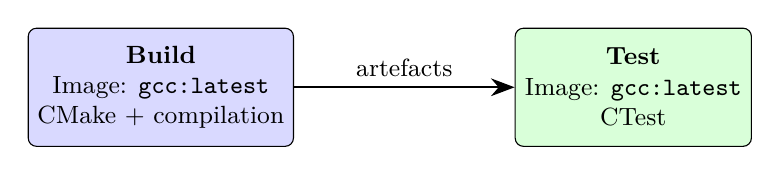
\begin{tikzpicture}[
  stage/.style={rectangle, draw, rounded corners=3pt, minimum width=3cm, minimum height=1.5cm, align=center, font=\small},
  arrow/.style={-{Stealth[length=3mm]}, thick}
]
  \node[stage, fill=blue!15] (build) at (0, 0) {\textbf{Build}\\Image: \texttt{gcc:latest}\\CMake + compilation};
  \node[stage, fill=green!15] (test) at (6, 0) {\textbf{Test}\\Image: \texttt{gcc:latest}\\CTest};

  \draw[arrow] (build) -- node[above, font=\small] {artefacts} (test);
\end{tikzpicture}
\end{center}

%% ============================================================
%% SECTION 13 : PROBLEMES RENCONTRES
%% ============================================================
\subsection{13. Problemes rencontres et solutions}\label{problemes-rencontres}

Cette section documente les principaux problemes techniques rencontres au cours du developpement, identifies a partir de l'historique Git et des sessions de debogage.

\subsubsection{13.1 Performance catastrophique : 2 min/epoque au lieu de 5 s}\label{perf-catastrophique}

\textbf{Symptome :} L'entrainement prenait environ 2 minutes par epoque au lieu des 5 secondes attendues.

\textbf{Cause :} La variable \texttt{CMAKE\_BUILD\_TYPE} n'etait pas definie, ce qui entrainait une compilation sans optimisations (equivalent a \texttt{-O0}). Sur un code a forte composante mathematique (produits matrice-vecteur, exponentielles), l'absence d'optimisations du compilateur a un impact dramatique.

\textbf{Solution :} Configuration explicite des drapeaux d'optimisation par compilateur, actives en configuration \texttt{Release} (via des expressions de generateur CMake) :

\begin{Shaded}
\begin{Highlighting}[]
\CommentTok{// MSVC : /O2 /fp:fast en Release}
\CommentTok{// GCC  : -O3 -ffast-math -march=native en Release}
\end{Highlighting}
\end{Shaded}

\textbf{Impact :} Acceleration d'environ \textbf{24x} (de $\sim$120s a $\sim$5s par epoque).

\subsubsection{13.2 Temps de chargement MNIST excessif}\label{chargement-lent}

\textbf{Symptome :} Le chargement du dataset MNIST prenait \textbf{plus de 8 minutes} a chaque lancement, rendant le developpement iteratif extremement lent.

\textbf{Cause :} Chaque lancement necessitait le chargement de 70\,000 fichiers PNG individuels, impliquant autant d'ouvertures de fichiers et de decompressions PNG.

\textbf{Solution :} Implementation d'un systeme de \textbf{cache binaire} (voir section 9.4). Lors du premier chargement, le dataset est sauvegarde en format binaire brut. Les lancements suivants chargent directement le cache binaire en un seul appel \texttt{fread()}.

\textbf{Impact :} Chargement reduit a \textbf{quelques secondes} ($\sim$100x plus rapide).

\subsubsection{13.3 Floating Point Exception lors du shuffle}\label{fpe-shuffle}

\textbf{Symptome :} Crash aleatoire avec une \emph{Floating Point Exception} lors du melange du dataset.

\textbf{Cause :} L'appel \texttt{rand() \% 0} lorsque le dataset etait vide (\texttt{count == 0}) provoquait une division par zero.

\textbf{Solution :} Ajout d'une verification en entree de la fonction \texttt{mnist\_shuffle()} :

\begin{Shaded}
\begin{Highlighting}[]
\ControlFlowTok{if} \OperatorTok{(!}\NormalTok{dataset }\OperatorTok{||}\NormalTok{ dataset}\OperatorTok{{-}\textgreater{}}\NormalTok{count }\OperatorTok{==} \DecValTok{0}\OperatorTok{)} \ControlFlowTok{return}\OperatorTok{;}
\end{Highlighting}
\end{Shaded}

\subsubsection{13.4 Divergence de la loss (NaN)}\label{loss-nan}

\textbf{Symptome :} La valeur de la loss devenait \texttt{NaN} apres quelques epoques d'entrainement.

\textbf{Cause :} Absence de stabilite numerique dans le calcul du softmax, combinee a un learning rate trop eleve.

\textbf{Solution :}
\begin{itemize}
\tightlist
\item Softmax recentre par le maximum : \(\text{softmax}(z)_i = \frac{e^{z_i - m}}{\sum_j e^{z_j - m}}\)
\item Clampage des probabilites avant \texttt{log()} : \texttt{max(p, $\varepsilon$)}
\item Clampage des entrees de la sigmoide dans \([-500, 500]\)
\end{itemize}

\subsubsection{13.5 Gradient vanishing avec Sigmoid}\label{gradient-vanishing}

\textbf{Symptome :} Sur des architectures a plus de 2 couches cachees, l'entrainement avec Sigmoid stagnait rapidement.

\textbf{Cause :} La derivee de la sigmoide est bornee par 0.25, ce qui provoque une attenuation exponentielle des gradients a travers les couches.

\textbf{Solution :} Utilisation de ReLU pour les couches cachees (derivee = 1 si actif), tout en conservant Softmax pour la couche de sortie. Cette combinaison ReLU/Softmax avec cross-entropy a permis d'atteindre \textbf{96\% de precision} contre 95\% avec Sigmoid/MSE.

\subsubsection{13.6 Allocations memoire dans la boucle d'entrainement}\label{allocations-boucle}

\textbf{Symptome :} Profilage (via \texttt{valgrind}) revelant 5.4 millions d'appels \texttt{malloc/free} pendant l'entrainement.

\textbf{Cause :} Les vecteurs de deltas et de gradients etaient alloues et liberes a chaque iteration de la boucle d'entrainement.

\textbf{Solution :} Pre-allocation de tous les buffers de travail lors de la creation du reseau et utilisation de la technique \textbf{ping-pong buffers} (voir section 8.2) pour alterner entre deux buffers pre-alloues sans aucune allocation dynamique.

%% ============================================================
%% SECTION 14 : CONFIGURATIONS D'ENTRAINEMENT
%% ============================================================
\subsection{14. Configurations d'entrainement}\label{configurations-entrainement}

Plusieurs configurations d'entrainement sont fournies dans le dossier \texttt{examples/}, permettant de comparer differentes combinaisons d'activations, de fonctions de perte et d'optimiseurs :

{\def\LTcaptype{none}
\begin{longtable}[]{@{}llll@{}}
\toprule\noalign{}
Exemple & Activation & Perte & Optimiseur \\
\midrule\noalign{}
\endhead
\bottomrule\noalign{}
\endlastfoot
\texttt{mnist\_train.c} & Sigmoid & MSE & SGD \\
\texttt{mnist\_train\_sigmoid\_sgd\_mse.c} & Sigmoid & MSE & SGD \\
\texttt{mnist\_train\_relu\_softmax\_adam\_cce.c} & ReLU / Softmax & CCE & Adam \\
\texttt{mnist\_train\_tanh\_softmax\_sgd\_cce.c} & Tanh / Softmax & CCE & SGD \\
\texttt{mnist\_train\_architectures.c} & Sigmoid & MSE & SGD (compare architectures) \\
\end{longtable}
}

%% ============================================================
%% SECTION 15 : PERFORMANCE ET BENCHMARKS (DARIS -- NE PAS MODIFIER)
%% ============================================================
\subsection{15. Performance et benchmarks}\label{performance-benchmarks}

Tous les benchmarks de cette section ont ete mesures sur un \textbf{ordinateur portable} equipe d'un processeur \textbf{Intel Core i5-12500H} (12 coeurs / 16 threads, 2.5--4.5 GHz) avec \textbf{16 Go de RAM DDR4}. La compilation est effectuee avec MSVC en mode Release (\texttt{/O2 /fp:fast}). Le programme utilise un seul thread (pas de parallelisation).

\subsubsection{15.1 Timing par architecture (5 epochs, Release build)}\label{timing-architecture}

{\def\LTcaptype{none}
\begin{longtable}[]{@{}lll@{}}
\toprule\noalign{}
Architecture & Temps/epoque & Samples/sec \\
\midrule\noalign{}
\endhead
\bottomrule\noalign{}
\endlastfoot
784$\to$128$\to$10 & 5s & 12\,000 \\
784$\to$256$\to$128$\to$10 & 12s & 5\,000 \\
784$\to$512$\to$256$\to$128$\to$10 & 30s & 2\,000 \\
\end{longtable}
}

\subsubsection{15.2 Debug vs Release}\label{debug-vs-release}

{\def\LTcaptype{none}
\begin{longtable}[]{@{}ll@{}}
\toprule\noalign{}
Build & Temps/epoque \\
\midrule\noalign{}
\endhead
\bottomrule\noalign{}
\endlastfoot
Debug (-O0) & $\sim$120s \\
Release (-O3) & $\sim$5s \\
\textbf{Ratio} & \textbf{$\sim$24$\times$} \\
\end{longtable}
}

\subsubsection{15.3 Precision MNIST}\label{accuracy-mnist}

{\def\LTcaptype{none}
\begin{longtable}[]{@{}ll@{}}
\toprule\noalign{}
Architecture & Precision test (5 epoques) \\
\midrule\noalign{}
\endhead
\bottomrule\noalign{}
\endlastfoot
784$\to$128$\to$10 & 93\% \\
784$\to$256$\to$128$\to$10 & 95\% \\
784$\to$512$\to$256$\to$128$\to$10 & 96\% \\
\end{longtable}
}

\subsubsection{15.4 Impact shuffle optimization}\label{impact-shuffle}

{\def\LTcaptype{none}
\begin{longtable}[]{@{}lll@{}}
\toprule\noalign{}
Shuffle & Temps & Par epoque (ms) \\
\midrule\noalign{}
\endhead
\bottomrule\noalign{}
\endlastfoot
Element par element & 53s & 88 \\
memcpy & 51s & 84 \\
Gain & \textbf{$\sim$3.9\%} & \textbf{$\sim$4.5\%} \\
\end{longtable}
}

\subsubsection{15.5 Comparaison optimiseurs (12s/epoque)}\label{comparaison-optimiseurs}

{\def\LTcaptype{none}
\begin{longtable}[]{@{}lll@{}}
\toprule\noalign{}
& SGD & Adam \\
\midrule\noalign{}
\endhead
\bottomrule\noalign{}
\endlastfoot
Temps/epoque & 12.0s & 12.3s \\
Memoire & Baseline & +2$\times$W \\
Precision finale & 95\% & 96\% \\
\end{longtable}
}

%% ============================================================
%% SECTION 16 : CONCLUSIONS
%% ============================================================
\subsection{16. Conclusions}\label{conclusions}

\subsubsection{Realisations}\label{realisations}

\begin{enumerate}
\def\labelenumi{\arabic{enumi}.}
\tightlist
\item
  \textbf{Implementation mathematiquement rigoureuse} de reseaux de neurones denses en C pur :
  \begin{itemize}
  \tightlist
  \item Propagation avant avec caches pre-alloues
  \item Retropropagation complete avec ping-pong buffers
  \item 6 fonctions d'activation, 4 fonctions de perte, 2 optimiseurs
  \end{itemize}
\item
  \textbf{Performances elevees} pour du C pur sans bibliotheque externe :
  \begin{itemize}
  \tightlist
  \item $\sim$12\,000 samples/sec sur architecture moyenne
  \item $\sim$24$\times$ d'acceleration Release vs Debug
  \item 93--96\% de precision MNIST en 5 epoques selon l'architecture
  \end{itemize}
\item
  \textbf{Interface web fonctionnelle} avec inference en temps reel :
  \begin{itemize}
  \tightlist
  \item Serveur Go avec chargement du modele binaire C
  \item Preprocessing cote client reproduisant la normalisation MNIST
  \item Affichage des probabilites par classe
  \end{itemize}
\item
  \textbf{Infrastructure de developpement complete} :
  \begin{itemize}
  \tightlist
  \item Pipeline CI/CD GitLab automatise (build + tests)
  \item 5 suites de tests (unitaires et integration)
  \item Build multi-plateforme (Linux, macOS, Windows)
  \end{itemize}
\end{enumerate}

\subsubsection{Limitations}\label{limitations}

\begin{itemize}
\tightlist
\item Single-thread SGD (pas de batching, pas de GPU)
\item Architectures dense-only (pas de convolution)
\item Pas de regularisation (dropout, L2)
\item Pas d'early stopping
\end{itemize}

\subsubsection{Travaux futurs}\label{travaux-futurs}

\begin{itemize}
\tightlist
\item Mini-batching pour ameliorer l'efficacite
\item Parallelisation OpenMP des produits matrice-vecteur
\item Support GPU (CUDA/OpenCL)
\item Architectures convolutives
\item Regularisation et dropout
\end{itemize}

\end{document}
